%%% Local Variables:
%%% mode: latex
%%% TeX-master: t
%%% End:

%\documentclass[bachelor,nofonts]{thuthesis}
\documentclass[master]{thuthesis}
%\documentclass[doctor]{thuthesis}
% \documentclass[%
%   bachelor|master|doctor|postdoctor, % mandatory option
%   winfonts|nofonts|adobefonts, % mandatory only for bachelor and Linuxer
%   secret,
%   openany|openright,
%   arialtoc,arialtitle]{thuthesis}
% 当使用 XeLaTeX 编译时,本科生、Linux 用户需要加上 nofonts 选项;
% 当使用 PDFLaTeX 编译时,adobefonts 选项等效于 winfonts 选项(缺省选项)。

% 所有其它可能用到的包都统一放到这里了,可以根据自己的实际添加或者删除。
\usepackage{thutils}

% 你可以在这里修改配置文件中的定义,导言区可以使用中文。
% \def\myname{薛瑞尼}

\begin{document}

% 定义所有的eps文件在 figures 子目录下
\graphicspath{{figures/}}


%%% 封面部分
\frontmatter

%%% Local Variables:
%%% mode: latex
%%% TeX-master: t
%%% End:
\secretlevel{绝密} \secretyear{2100}

\ctitle{基于命名数据网络的服务中心网络设计与实现}
% 根据自己的情况选,不用这样复杂
\makeatletter
\ifthu@bachelor\relax\else
  \ifthu@doctor
    \cdegree{工学博士}
  \else
    \ifthu@master
      \cdegree{工学硕士}
    \fi
  \fi
\fi
\makeatother


\cdepartment[计算机]{计算机科学与技术系}
\cmajor{计算机科学与技术}
\cauthor{陈硕} 
\csupervisor{曹军威副研究员}
% 如果没有副指导老师或者联合指导老师,把下面两行相应的删除即可。
%\cassosupervisor{陈文光教授}
%\ccosupervisor{某某某教授}
% 日期自动生成,如果你要自己写就改这个cdate
%\cdate{\CJKdigits{\the\year}年\CJKnumber{\the\month}月}

% 博士后部分
% \cfirstdiscipline{计算机科学与技术}
% \cseconddiscipline{系统结构}
% \postdoctordate{2009年7月——2011年7月}

\etitle{An Design of Service Network Based on Naming mechanism} 
% 这块比较复杂,需要分情况讨论:
% 1. 学术型硕士
%    \edegree:必须为Master of Arts或Master of Science(注意大小写)
%              “哲学、文学、历史学、法学、教育学、艺术学门类,公共管理学科
%               填写Master of Arts,其它填写Master of Science”
%    \emajor:“获得一级学科授权的学科填写一级学科名称,其它填写二级学科名称”
% 2. 专业型硕士
%    \edegree:“填写专业学位英文名称全称”
%    \emajor:“工程硕士填写工程领域,其它专业学位不填写此项”
% 3. 学术型博士
%    \edegree:Doctor of Philosophy(注意大小写)
%    \emajor:“获得一级学科授权的学科填写一级学科名称,其它填写二级学科名称”
% 4. 专业型博士
%    \edegree:“填写专业学位英文名称全称”
%    \emajor:不填写此项
\edegree{Master of Engineering} 
\emajor{Control Science and Engineering} 
\eauthor{Chen Shuo} 
\esupervisor{Associate Professor Cao Junwei} 
%\eassosupervisor{Chen Wenguang} 
% 这个日期也会自动生成,你要改么?
% \edate{December, 2005}

% 定义中英文摘要和关键字
\begin{cabstract}
   近年来,互联网基础设施及应用服务快速发展,互联网“基础架构化”的趋势明显。在私有的分布式系统内部,服务多以服务接口的形式进行集成。在全局互联网中,越来越多的网络资源服务如Amazon云存储,微信公共账号等以SOAP(Simple Object Access protocol)或者REST(Representational State Transfer)接口的形式对外提供服务。而近些年云计算的发展与推广,使基于云服务尤其软件即服务(Software as a Service,SAAS)的接口服务得到大规模普及。

   SOAP和REST为当前最流行的两种Web Service服务形式。REST需要基于下层的HTTP协议。SOAP虽然对下层协议没有特定的限制,但是HTTP协议是最普遍的实现方式。HTTP协议也成为了事实上的网络瘦腰(narrow waist)。而从HTTP协议开始,自上而下需要经过多层协议栈,而各层协议栈为了通用性没有对大规模的服务网络进行优化。HTTP协议以目标主机名为基础对数据包进行命名。近些年来,信息中心网络作为一种新的网络架构设计范式被提出来。其核心是以内容命名网络包来取代以地址命名的网络包。以其中的命名服务网络为例,以命名数据包替代IP网络包作为新的网络瘦腰。将服务网络与命名数据网络的性质有机结合起来,为服务网络从底层进行优化提供了新的研究方向。本文中,作者通过命名机制,提出一种重构面向服务的网络协议栈设计,并对该设计的协议性能,安全性等进行实验研究,最后提出一种将该服务网络应用于局部分布式系统的方案。作者的主要工作是:

  \begin{itemize}
    \item 开发一种基于命名服务网络的存储软件,并以此软件为原型提出基于命名机制的服务网络设计原则;
    \item 提出一种基于命名机制的服务网络协议设计即命名服务网络;
    \item 对命名服务网络原型进行实现,并对该网络服务进行多方位实验测试;
    \item 提出一种基于命名服务网络的服务设计方案。
  \end{itemize}
\end{cabstract}

\ckeywords{Web Service, 信息中心网络, 命名数据网络}

\begin{eabstract} 
   Internet infrastructure and overlay services have been widely deployed in recent years. The trend of infrastructuralization of Internet has been increasingly apparent. In local system, distributed services are commonly integrated with remote control interfaces. In Internet, more and more services or functions, for example Amazon EC2, Wechat public account, are provided in the form of SOAP or REST apis. As cloud services are drawing more attentions, cloud services, especially based on SAAS, are becoming more popular.

   SOAP and REST are two most widely used Web Service protocol. REST works upon HTTP. SOAP are not binded with specific protocol, while HTTP is the most common underlying protocol. HTTP is the de facto network narrow waist. Web services are over multiple layers of network stacks, which are not optimized for service efficiency. The web service network packet is actually in the form of HTTP packet. In recent years, Informaction Centric Network (ICN) is proposed as new network architecture pattern. Named Data Network (NDN), for example, replaces IP packet with named data packet as new network narrow waist. Combining web service with ICN shows new perspective of optimization. In this paper, a new design of service network based on naming mechanism is proposed. Performance, security and etc. are evaluated. A framework of distributed system based on named service networking is also discussed. The main work of this dissertation is as follows:

   \begin{itemize}
    \item A data repository of NDN is devloped. Principles of Named Service Network are proposed based on this prototype.
    \item Details of Named Service Network (NSN) are demonstrated.
    \item Prototyple of NSN is developed. Evaluation of NSN is conducted.
    \item An implementation of NSN on distributed system is provided.
  \end{itemize}
   
\end{eabstract}

\ekeywords{Web Service, Information Centric Networking, Named Data Networking}

% 设置 PDF 文档的作者、主题等属性
\makeatletter
\thu@setup@pdfinfo
\makeatother
\makecover

% 目录
\tableofcontents

% 符号对照表
%\begin{denotation}

\item[HPC] 高性能计算 (High Performance Computing)
\item[cluster] 集群
\item[Itanium] 安腾
\item[SMP] 对称多处理
\item[API] 应用程序编程接口
\item[PI]	聚酰亚胺
\item[MPI]	聚酰亚胺模型化合物,N-苯基邻苯酰亚胺
\item[PBI]	聚苯并咪唑
\item[MPBI]	聚苯并咪唑模型化合物,N-苯基苯并咪唑
\item[PY]	聚吡咙
\item[PMDA-BDA]	均苯四酸二酐与联苯四胺合成的聚吡咙薄膜
\item[$\Delta G$]  	活化自由能~(Activation Free Energy)
\item [$\chi$] 传输系数~(Transmission Coefficient)
\item[$E$] 能量
\item[$m$] 质量
\item[$c$] 光速
\item[$P$] 概率
\item[$T$] 时间
\item[$v$] 速度
\item[劝  学] 君子曰:学不可以已。青,取之于蓝,而青于蓝;冰,水为之,而寒于水。
  木直中绳。(车柔)以为轮,其曲中规。虽有槁暴,不复挺者,(车柔)使之然也。故木
  受绳则直, 金就砺则利,君子博学而日参省乎己,则知明而行无过矣。吾尝终日而思
  矣,  不如须臾之所学也;吾尝(足齐)而望矣,不如登高之博见也。登高而招,臂非加
  长也,  而见者远;  顺风而呼,  声非加疾也,而闻者彰。假舆马者,非利足也,而致
  千里;假舟楫者,非能水也,而绝江河,  君子生非异也,善假于物也。积土成山,风雨
  兴焉;积水成渊,蛟龙生焉;积善成德,而神明自得,圣心备焉。故不积跬步,无以至千
  里;不积小流,无以成江海。骐骥一跃,不能十步;驽马十驾,功在不舍。锲而舍之,朽
  木不折;  锲而不舍,金石可镂。蚓无爪牙之利,筋骨之强,上食埃土,下饮黄泉,用心
  一也。蟹六跪而二螯,非蛇鳝之穴无可寄托者,用心躁也。\pozhehao{} 荀况
\end{denotation}



%%% 正文部分
\mainmatter

%%% Local Variables:
%%% mode: latex
%%% TeX-master: t
%%% End:

\chapter{引言}
\label{cha:intro}
\section{研究背景}
\subsection{Web Service}
随着20世纪90年代互联网技术的快速发展以及电子商务大规模部署,企业级软件也从大规模集中的复杂软件向分布式松耦合的Web服务进化。SOA(service-oriented architecture, 面向服务体系架构)作为一种新的软件设计概念被提出来。虽然没有对SOA统一的确定性定义,但普遍指一种基于开放的协议或标准,将松耦合、自治的功能服务进行整合的设计思想。而随着面向服务的网络服务设计思想的普及,一些企业联盟及组织也制订了Web服务的通用标准与协议。W3C组织将Web服务(Web Service)定义为支持通过网络机器之间互操作的软件系统。\cite{haas2004web}同时工业界逐渐接收基于SOAP(Simple Object Access Protocol)协议的Web Service架构。
\subsubsection{SOAP服务架构概述}
SOAP协议指简易对象访问协议。在Web Service架构中作为格式化信息交换协议。SOAP协议定义类以XML格式为基础的数据封装格式,定义了数据格式,远程调用与应答的封装。SOAP协议虽然不限制下层的通信协议,但是普遍采用HTTP协议与当前浏览器兼容。以SOAP协议为基础,Web Service的三大组件分别为SOAP,WSDL(Web Services Description Language,网络服务描述语言)及UDDI(Universal Description Discovery and Integration,统一描述、发现和集成协议)。WSDL是基于XML用来描述Web Service服务的文档语言。通过WSDL文档以规定Web Service所执行的操作,使用的消息,数据类型以及需要绑定的通信协议。UDDI提供了一种Web Service的目录服务,提供了一种通过Internet来注册Web Service信息,来促进Web Service互相发现与利用的检索与集成服务。

一个典型的Web Service如图\ref{fig:web-service-arc}所示。服务请求者和服务提供者通过SOAP协议进行通信。而服务提供者将服务描述注册到服务协调者UDDI上。服务请求者可以通过服务协调者获得该服务的操作接口,也可以对多个服务进行服务组合。
\begin{figure}[H]
  \centering
  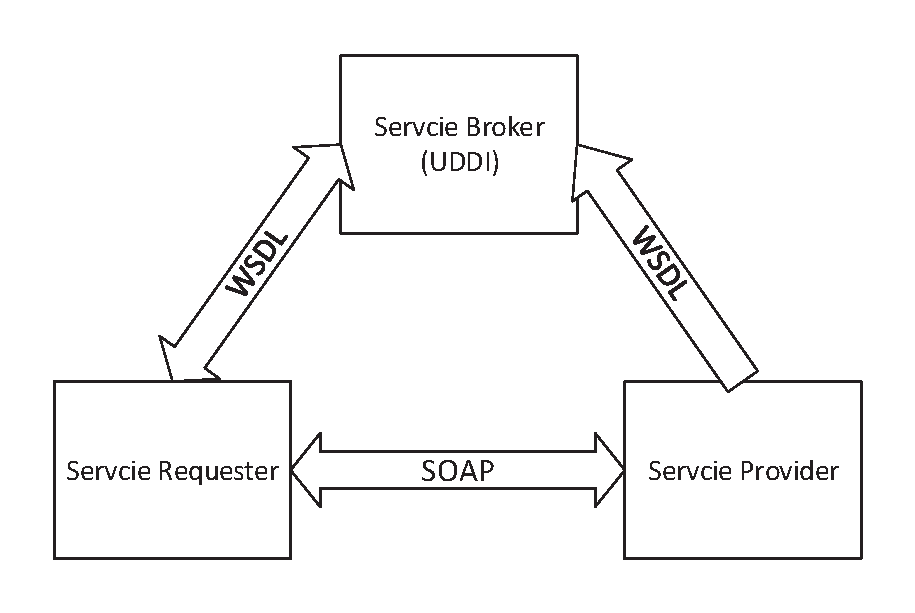
\includegraphics[width=0.6\textwidth]{web-service-arc}
  \caption{Web Service典型架构}
  \label{fig:web-service-arc}
\end{figure}

\subsubsection{REST服务架构概述}
REST(Representational state transfer)并不是特指具体一种通信协议,而是一种扩展服务设计的原则。随着近些年云服务的开展普及,REST在工业界得到了非常广泛的应用,如Amazon S3,微信公共账号接口等。与SOAP协议不同,REST需要直接利用HTTP协议作为传输协议,利用HTTP动词(GET,POST,PUT,DELETE)与URI的组合来定义REST的具体服务操作。

\subsubsection{存在的问题}

对于当前最普遍的两种Web服务架构即基于SOAP与REST普遍是现在HTTP协议之上。在SOAP中,包含服务请求与应答的XML报文直接封装在HTTP数据包之中。在REST中,资源直接通过HTTP的URI进行标记,通过HTTP动词对资源进行操作。HTTP协议已经成为事实上的网络瘦腰(narrw waist)。\cite{popa2010http}但以HTTP为承载的服务网络包含如下问题:HTTP为应用层协议,到物理层信号传输还要经过多层次的协议栈。而相关的经典协议栈如IP协议、以太网协议等兼顾通用性,未对事实上的瘦腰HTTP协议进行优化。例如HTTP协议无法阻止在底层网络层面阻止DDOS攻击,网络层面无法直接缓存数据包,需要服务提供商自建或租用CDN系统。REST架构的网络服务中,本质是面向资源,面向内容的状态控制变化的,客户端不需要关心服务或资源的具体位置。而当前底层最普遍的IP网络是面向连接的,在处理相同资源在不同的物理地址路由时,无法做到面向内容的优化路由。

\subsection{信息中心网络概述}

随着当今互联网数据分发流量的快速增长,TCP/IP架构在内容分发方面暴露出一些问题。因此信息中心网络(Information Centric Networking,ICN)作为一种新的网络架构设计原则被提出来。目前正在积极研究并开发的ICN网络项目有:DONA(Data-Oriented Network Architecture)\cite{koponen2007data},Named Data Networking(NDN)\cite{jacobson2009networking},Content-Centric Networking(CCN)\cite{jacobson2009networking},Publish-Subscribe Internet Routing Paradigm(PRISP)\cite{ain2009d2},Network of Information(NetInf)\cite{ahlgren2010second}等。虽然实现方式细节上各有不同,但是设计目标与架构特点相似。都是为了更有效率地获取与分发数据,并解决网络中断,流量洪泛等问题。网络通信通常由数据请求端驱动。网络包单位为命名数据对象(named data object,NDO)。\cite{ahlgren2012survey}ICN对于传统的TCP/IP架构网络的颠覆则是利用NDO来替代IP包作为新的网络瘦腰。

\section{研究内容及意义}
本论文主要研究利用信息中心网络的命名数据机制设计一种新的面向服务的网络架构,并对该架构进行原型实现与实验评估。具体研究内容为:
\begin{itemize}
\item 提出一种基于命名机制的服务网络协议设计,即命名服务网络协议;
\item 以命名服务网络协议为基础设计一套服务网络架构,包括服务发现,服务路由,安全验证,服务仲裁等组件
\item 提出一套服务网络比较框架,并与SOAP与REST的网络服务架构进行比较分析
\item 根据命名服务网络架构设计一种本地分布式计算系统方案
\end{itemize}
研究意义在于打破传统服务网络基于HTTP协议与TCP/IP面向连接的网络架构,充分利用信息中心网络的性质特点提出一种新的网络设计范式,并未未来服务网络实现提供一种可能方案。
\section{章节安排}
本论文公分7章,各章内容如下:

第一章介绍课题的背景与研究意义。

第二章介绍本文涉及到的服务网络包括Web Service以及信息中心网络的基本概况与研究进展。重点介绍命名数据网络的架构以及当前的开发动态。同时多种介绍基于信息中心网络的服务架构研究,分析比较各个研究特点并总结不足。

第三章介绍作者参与的基于命名数据网络存储软件的开发细节,并总结出基于命名数据网络服务开发的原则。

第四章介绍命名服务网络的协议与架构设计。

第五章进行命名服务网络的原型实现,并基于该原型进行实验评估。

第六章提出一种基于命名服务网络的本地分布式服务集群设计

第七章对前面所做工作进行总结并指出未来需要完善的工作,并对未来研究做出展望。



%%% Local Variables: 
%%% mode: latex
%%% TeX-master: t
%%% End: 

\chapter{相关工作}
\section{Web Service相关研究概述}
Web服务从广义上指基于网络的主机与主机之间互操作的软件系统。Web服务的主要特点在于提供轻量级的Web调用接口提供自足的(self-contained)松耦合的服务。狭义Web服务特指Web Service类似于W3C制定的基于SOAP协议的服务架构。该架构最基本的元素如引言所述的SOAP+WSDL+UDDI。关于Web Service架构的研究与应用开发在21世纪伊始比较热,而最近大与服务提供商更加倾向于使用形式上更加简单的REST接口。
\subsection{基于SOAP协议的Web Service}
\subsubsection{服务架构}
与工业界注重W3C及企业联盟注重标准制定与协议规范不同,学术界更加注重以通信协议为基础如何解决在资源动态变化的基础上解决日益复杂的应用需求。研究的问题主要包括Web数据集成、服务组合、访问控制、事件机制以及语义网(semantic web)相关研究。一个最基本的Web Service架构如图\ref{fig:web-service-arc-2}所示。

\begin{figure}[H]
  \centering
  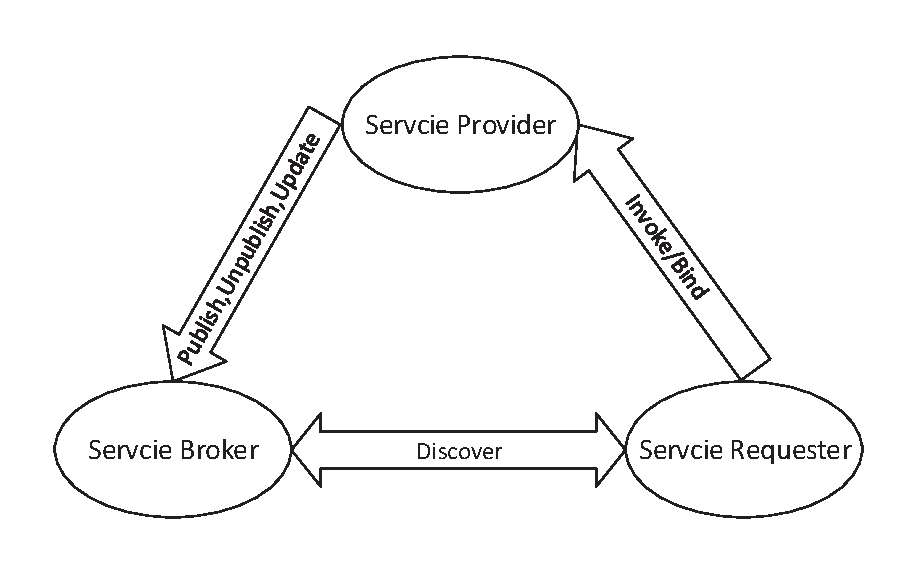
\includegraphics[width=0.6\textwidth]{web-service-arc-2}
  \caption{Web Service模型架构}
  \label{fig:web-service-arc-2}
\end{figure}

Bussler\cite{fensel2002web}指出由UDDI,WSDL和SOAP组成的协议栈无法实现真正可扩展的广域Web Service服务。实现可扩展的Web服务发现,选择,协调以及组合需要包含以下最基本的元素\cite{bussler2001b2b}:
\begin{itemize}
\item 文档类型(Document Types):文档类型为交换文档的基本语义。即文档类型定义了服务请求者与服务提供者数据交换的格式以及需要采取的语义(semantics)。
\item 语义(semantics):服务提供者与服务请求者确定相同的文档类型并保证传递信息语义的正确。因此需要语义词典来枚举文档元素所有可能的可用值。本体论(ontology)提供了一种对数据概念定义的一种手段,以保证对于数据概念解释的一致性。
\item 相关传输协议:服务请求双方需要约定好一致的通信协议。针对SOAP协议,底层协议可以为HTTP,SMTP,TCP,UDP或者JMS。
\item 信息交换序列:由于底层交换信息未必是可靠传输,可能发生报文重传与丢失现象,所以需要对交换报文添加序列号或消息确认以保证交换信息的完整性。
\item 流程:对于一个完整的服务而言,一次服务信息交换未必能够完成指定服务。例如一次购买行为,需要先将商品加入购物车,确定订单之后付款。之间至少需要三次服务请求双方的信息交换,并且顺序不能颠倒。所以服务双方需要确定一套服务协议流程。
\item 安全:安全性即服务最基本的需求,包括保证报文的私密性以及完整性。再次基础上还有服务与资源的访问控制等问题
\item 句法:即文档格式,如XML,JSON等
\item 服务配置:在各个相关服务端进行交互之前,可能服务主机的配置不相同,例如语义词典,服务流程等。当双方开始进行交互时,需要根据服务端进行特定配置。
\end{itemize}

文献\cite{fensel2002web}提出Web服务建模框架(Web Service Modeling Framework,WSMF)。WSMF旨在提出一套完全灵活并可扩展的Web服务架构。W3C也以WSMF框架为基础发布了一些列Web Service规范。\cite{WSMF-imp}WSMF架构。WSMF架构基于一下两个原则:元件,元素之间的强解耦性;强中介性,任何元素或服务之间可以通过扩展方式进行相互对话,强调元素与目标的的重用性及语义。WSMF的十字形架构如图\ref{fig:WSMF-arc}所示。图\ref{fig:WSMF-arc}采用文献\cite{WSMF-imp}的改进“十字形模型”。

\begin{figure}[H]
  \centering
  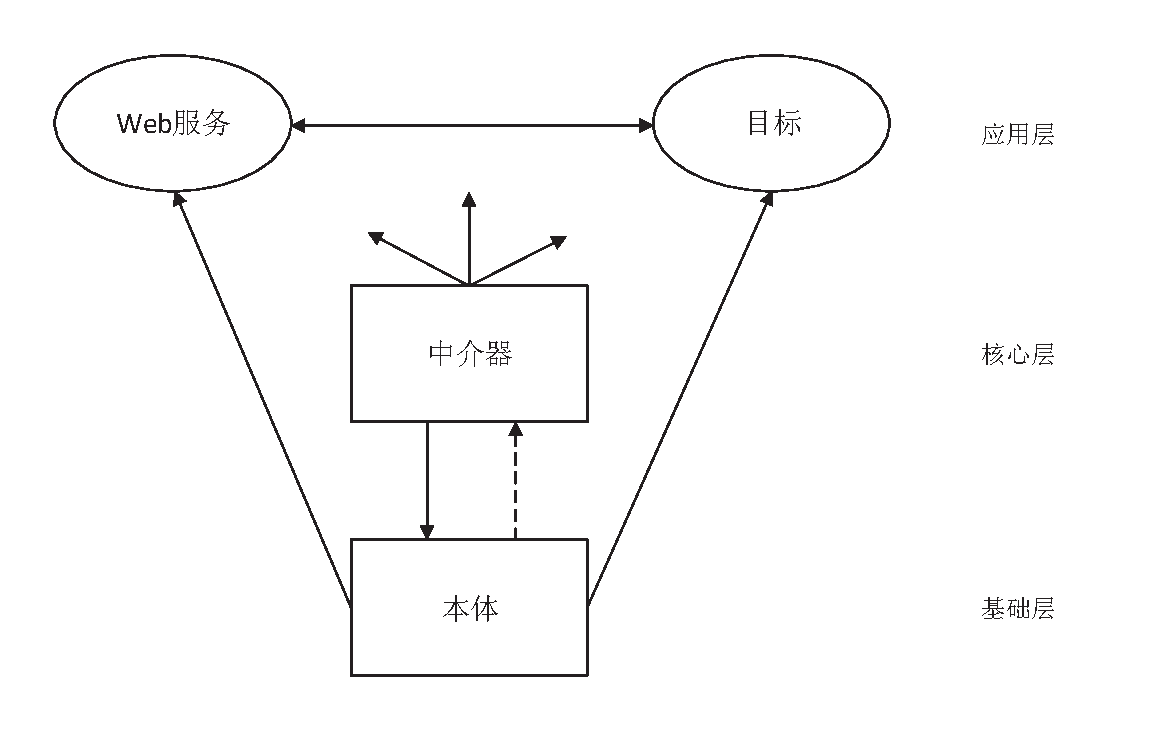
\includegraphics[width=0.7\textwidth]{WSMF-arc}
  \caption{WSMF顶层要素与相互关系}
  \label{fig:WSMF-arc}
\end{figure}

该模型中应用层为各种可被重用的任务集$\{\mathrm{WS}\mid\mathnormal{ws_{1}}, \mathnormal{ws_{2}}, \mathnormal{ws_{3}} \cdots \mathnormal{ws_{m}}\}$ 与$ \{\mathrm{G}\mid\mathnormal{g_{1}}, \mathnormal{g_{2}}, \mathnormal{g_{3}} \cdots \mathnormal{g_{n}}\}$。在具体实现相关应用时即为实现指定目标$\mathnormal{G_j}, \mathnormal{G_j}\subset\mathnormal{G}$而按一定流程重新组合$\mathnormal{W_i}, \mathnormal{W_i}\subset\mathnormal{W}$。

WSMF的核心为中介器,包括本体中介器,目标中介器,服务中介器,以及目标服务组着中介器。用来协调各个元素之间的组合关系。此外需要协调服务与服务之间包括传送协议,数据结构,信息格式的不同方言等问题。本体为WSMF架构的基础,对服务,目标,中介器进行描述和条件约束。

\subsubsection{服务发现}
在服务发现技术方面,服务发现是指服务请求者基于某单一既定目标查找选定需要的服务。工业界最常见的为UDDI服务,但依旧在更高的复杂性和信息组合自动化方面有所不足。当前Web服务发现的主要技术如表\ref{tab:web-service-discovery}所示。\cite{klein2001serching}

\begin{table}[htb]
  \centering
  \begin{minipage}[t]{0.8\linewidth}
  \caption{主流服务发现技术比较}
  \label{tab:web-service-discovery}
    \begin{tabular}{c	c	c	c}
      \toprule[1pt]
      \textbf{Service Discovery Technologies} & \textbf{Precision} & \textbf{Recall} & \textbf{Hardness} \\\midrule[0.5pt]
      Keyword Based & Low & High & Average\\
      Frame Based & High & Low & Average\\
      Deductive Retieval & High & High & Hard\\
      \bottomrule[1pt]
    \end{tabular}
  \end{minipage}
\end{table}

大多数检索方法是类似于基于UDDI的框架(Frame Based)方法。基于逻辑推导(Deductive Retieval)的方法由于服务在概念上与约束上非常难表述,所以实现难度最高。Mark Klein,Abraham Bernstein提出一套基于Ontology的服务发现架构,将服务描述通过语义网(Semantic Web)重新组织,提出了一套查询方式更加灵活,查询准确性更高的框架。\cite{klein2001serching}

\subsubsection{Web服务安全}
Web服务安全研究主要分为两个方面即,访问控制与数据安全。Web Service访问控制技术大体分为:
\begin{itemize}
\item 基于主机认证:基于访问主机请求中的网络认证信息(如hostname, IP等),缺点是无法控制区分同一主机的不同用户,信息也比较容易伪造。
\item 基本认证:基于辨识身份的用户名与密码,用户名与密码在基于HTTP的传输中保持为明文。
\item 基于SSL/TLS的身份证书:利用证书对传输信息进行加密或签名,是工业实现中相对可靠,并且主流的实现方式。而对证书的分发与信任模型(trust model)本身为密码工业的研究范围
\end{itemize}

WS-Security作为SOAP的扩展协议由OASIS于2002年提出。\cite{nadalin2002web}该协议旨在保证Web服务信息传输的加密型以及防止信息篡改。该协议支持多种安全信令包括X.509,Kerberos,以及 Security Assertion Markup Language(SAML),提供端到端的信息安全保护。

\subsection{基于REST的Web服务架构}
REST(表述性状态转移,Representational state transfer)不是指具体的某个协议,而是一种构建分布式可扩展web服务的最佳实践原则。REST通常通过HTTP协议来组织超媒体(Hypermedia)资源。

REST的主要设计原则为:
\begin{itemize}
\item 统一接口:通过HTTP动词(GET,POST,PUT,DELETE)对以URI标记的资源进行操作以代表创建,读取,更新,删除等操作
\item 自描述性:资源与其描述为松耦合,因此资源可以以不同的格式存在(XML,JPEG,PDF等)。客户端与服务端可以利用HTTP中对资源描述的元数据对资源进行操作
\item 无状态性:对于资源操作在服务端与客户端是无状态的。状态描述被显式的保存在超链接上。
\end{itemize}
以微信公共账号服务接口为例,采用REST风格的调用接口。通过服务号群发消息的接口如下:

\noindent
\fbox{
\parbox{0.9\textwidth}{
  \small{http请求方式: POST\\
  https://api.weixin.qq.com/cgi-bin/media/uploadnews?access\_token=ACCESS\_TOKEN}
 }
}

HTTP报文封装的POST的数据为JSON格式的一段文档。

一些组织也在进行基于REST的服务架构标准化工作,包括Open Mobile Alliance(OMA)以及IETF。OMA研究主要集中在基于Parlay-X(一种电话网络中Web Service的服务架构)REST接口研究与制定。\cite{alliancerestful}IETF也在制定基于REST的集中会议控制协议(Centralized Conferencing Manipulation Protocol,CCMP)\cite{barnes2009centralized}。

\section{信息中心网络相关研究概述}
\subsection{信息中心网络研究概述}
TCP/IP在早在20世纪70年代就被提了出来,当时网络的主要需求即为固定主机间端到端的可靠通信。且在简单IP层的瘦腰网络架构支持下,上层网络应用只要基于最简单的IP协议,即可在互联网上运行,所以大量的互联网创新应用随之而来。随着当今互联网越来越向数据分发的方向演进,以命名数据取代IP网络瘦腰的信息中心网络设计思想作为一种全新的架构被提出来。当前主要的ICN架构包括DONA,NDN,PRISP和NetInf。ICN设计主要考虑如下五个方面\cite{xylomenos2014survey}:

\begin{itemize}
\item 命名:在所有的ICN架构中,网络包的命名与主机地址无关。命名方式有两种,即扁平化或层次化的命名方式
\item 名字解析与数据路由:主要分为耦合和解耦两种方式。在耦合方式中,命名数据请求被转发到相应的主机后,数据沿着请求反向路径返回给数据请求者。在解耦方式中,数据应答的返回路径不做限制。
\item 缓存:缓存设计主要分为\textit{on-path}和\textit{off-path}两种。\textit{on-path}方式指的是数据被缓存在数据请求的转发路径上。\textit{off-path}缓存需要请求转发与路由系统支持,即缓存数据主机可以被当做正常的数据发布者
\item 移动:ICN天然地支持数据请求者的移动性,因为当请求链接失败之后,请求者可以在新的地点构建新的数据请求路径。而数据发布者的移动性支持较难,需要一定的路由机制重新更新请求路由转发表。
\item 安全:安全机制设计与数据命名方式直接相关。扁平的命名方式需要命名数据能够自验证,而结构化的命名方式则可以建立结构化的信任模型(trust model)。
\end{itemize}

\subsection{命名数据网络架构及研究进展}
本文中的命名服务网络设计主要基于ICN中的命名数据网络架构设计(Named Data Networking,NDN)。NDN架构在2009年由Van Jacobson等人提出。\cite{jacobson2009networking}NDN架构如图\ref{fig:IP-vs-NDN}所示。NDN的网络架构继承了IP架构的沙漏型瘦腰结构。由于瘦腰的简单性,上下层协议只要支持瘦腰协议即可进行大量创新,这个瘦腰架构也是互联网发展30年来的成功经验
。在NDN架构中利用命名数据包来取代以端主机地址标记的IP网络包。

\begin{figure}[H]
  \centering
  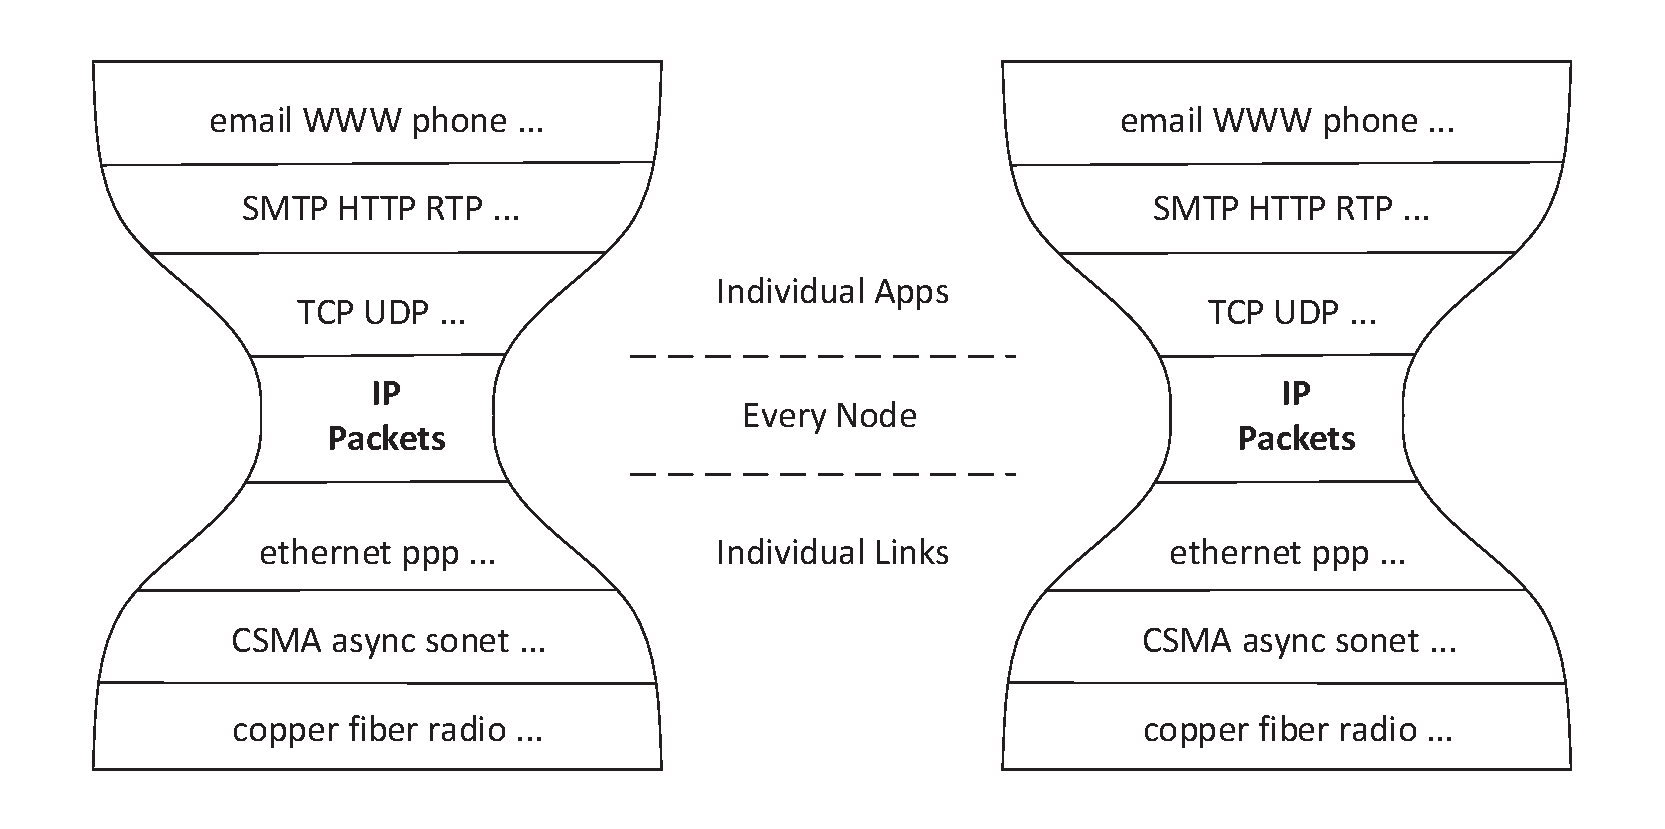
\includegraphics[width=0.9\textwidth]{IP-vs-NDN}
  \caption{IP与NDN架构对比}
  \label{fig:IP-vs-NDN}
\end{figure}

NDN的主要设计原则是:
\begin{itemize}
\item 命名:NDN采用结构化URI方式的命名。结构化的命名方式可以使路由更加具有扩展性,即可以采用名字前缀方式进行路由。命名方式不涉及网络上的信息如(IP地址)而是直接应用相关,即应用可以不依赖网络选择特定的命名方式。
\item 安全:安全特性在NDN架构的另一个基础。NDN架构采用以数据为中心的安全,及对每一个数据包单独进行签名。数据的安全性与数据在哪里存放解耦。
\item 名字解析与数据路由:名字解析不直接整合在NDN架构中,就像IP网络中DNS是独立的网络一样。NDN路由采用耦合方式,即数据会根据数据数据请求的转发路径反向转发。由于NDN采用前缀转发的方式与IP类似,所以NDN可以采用IP类似的BGP,IS-IS和OSPF转发协议。
\item 缓存:由于NDN采用耦合方式转发数据请求,数据可以被缓存在数据请求路径的中间节点上。而NDN与IP不同的是可以做到真正的网络层缓存。因为NDN数据包与IP数据包不同的是直接以应用数据名字命名,而不是以地址命名,所以在缓存中的数据可以被其他请求端重用。而由于NDN数据包的数据中心安全性,数据包缓存在网络中可以被加密也可以签名防止被篡改。
\item 智能数据平面:与IP不同,IP是一个无状态协议,路由器很难在IP的层面对路由状态进行监控。而NDN中的请求等待表(Pending Interest Table,PIT)记录了所转发数据请求的一些列转发状态信息。而抓发节点可以根据PIT所记录的软状态(soft state)构建智能的转发策略。
\end{itemize}

NDN数据包分两种,数据兴趣包(interest packet)与数据包(data packet),如图\ref{fig:NDN-packet}所示。兴趣包封装请求数据的名字以及一些其他选择条件。当兴趣包被转发到含有相应数据包的主机时,该节点可以返回相应的数据包。
\begin{figure}[H]
  \centering
  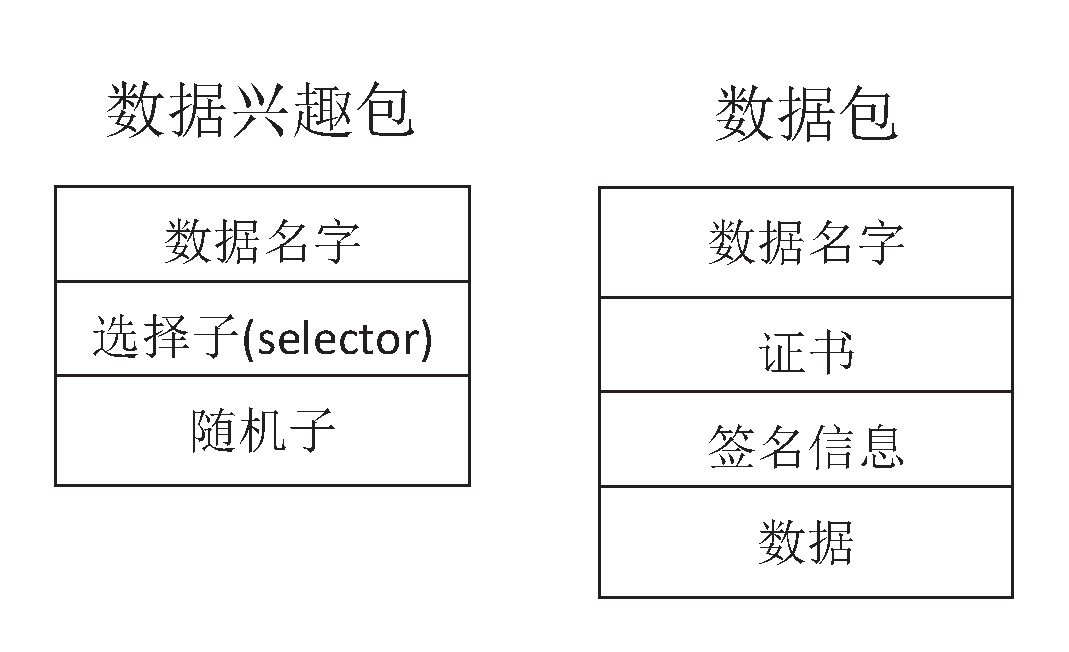
\includegraphics[width=0.7\textwidth]{NDN-packet}
  \caption{IP与NDN架构对比}
  \label{fig:NDN-packet}
\end{figure}

NDN协议处理架构主要是基于三个表即转发表(Forwarding Information Base,FIB),兴趣等待表(Pending Interest Table,PIT)与内容缓存(Content Store,CS)。FIB转发表类似于IP的转发表,用来存储名字前缀以及对应的转发接口。PIT表用来存储在本节点转发出去并且还没被相应的interest。CS表即内容缓存,用来缓存返回的数据包。

一个节点处理interest请求过程为,首先查找CS看是否有对应的数据包,如果有直接返回,如果没有则查找FIB表,看有没有转发的合适条目,如果存在则按照FIB规则转发,同时interest被存储在PIT中。当对应的请求包回到该节点时,一方面根据CS缓存策略对该数据包进行缓存,另一方面根据PIT表存储的interest信息返回该数据,并删除PIT表中的该条目。

\subsection{基于信息中心网络的服务网络相关研究}
ICN本质上是把传统网络中的\textit{where}模型转化为\textit{what}模型,网络直接处理的是应用数据的抽象。而一些研究在数据之上进一步地进行抽象,认为网络的本质是承载与连接服务。

文献\cite{nordstrom2012serval}提出一种服务中心网络协议栈(Serval)。通过ServiceID来标记应用网络包,通过FlowID用来标记当连接建立后的网络包。Serval协议栈中还增加了Service Table和Flow Table用来记录Service和Flow的网络状态,在Host端可以可以针对网络服务情况进行状态保持和只能决策。

文献\cite{braun2011service,braun2013service}中提出一种服务中心网络(Service-Centric Networking,SCN)架构以及一种基于NDN的服务中心网络实现。在沙漏架构中将NDN的命名数据包替换成服务对象。SCN修改Interest的结构使其能够封装服务请求参数。但整体来说SCN就是对NDN表述的重新抽象以及对流程的简单修改。

文献\cite{wu2014sofia}提出了一种基于ICN的面向服务信息网络架构(SOFIA)。而SOFIA的本质也是利用了NDN的命名、转发与缓存机制。此外在SOFIA中增加了Service Relay角色,相当于一种服务代理。服务请求者可以请求Service Relay在不同的网络环境中进行新的服务请求连接。这种机制有助于网络中multihoming,multicast以及mobility的实现。


%%% Local Variables: 
%%% mode: latex
%%% TeX-master: t
%%% End: 

\chapter{基于命名数据网络的存储服务}
\label{repo}

\section{命名数据网络存储原型介绍}
在NDN中,缓存结构(CS)直接集成在NDN的架构之中,但CS架构还不能完全满足复杂的内容操作要求:一方面CS只是数据的缓存,数据会被替换掉;另一方面对于数据的插入,删除,访问控制等问题,CS完全没有主动操作接口。NDN网络架构取代当前的IP网络架构的一个主要动机就是,当前网络最主要的流量是数据分发,NDN以数据为中心的拉模式(pull)也非常适合数据分发类的应用。

CS可以将数据直接存储在网络层,而相应数据存储应用也可以将数据存储在网络直接可操作的层面。NDN架构支持网络层次存储的的主要原因为:1.NDN直接以数据本身的名字进行命名。在IP网络中,数据以源地址和目的地址进行命名,数据无法被其他主机重用。虽然有组播的方式,但是对于组播组之外主机还是无法进行重用。2.数据隐私:每一个命名数据都带着签名,数据的非拥有者无法对数据进行篡改。同时数据发布者可以对数据直接进行加密,数据的私密性也可以得到保证。

在NDN中,数据仓库(repository,简称repo)为持久数据存储模型。在NDN中,NDN Repo的概念为被单一组织管理的运行在NDN网络上的数据存储应用。NDN Repo直接运行在NDN网络之上,而不是去修改NDN的底层协议。Repo最主要的作用就是为数据提供持久存储,处理NDN网络转发的数据请求(inerest)。Repo的存储单位为数据对象(data object),数据的管理单位为\textit{data object}的名字前缀。NDN Repo需要遵守NDN Repo协议,该协议定义了操作Repo的基本语义与流程。协议内容基本包括数据的插入,删除以及查询。Repo协议中为数据的访问控制,安全信任提供了框架,但是没有具体规定访问政策与信任模型。同时NDN Repo实现了应用层网络封装的概念。\cite{clark1990architectural}

同NDN直接的数据分发功能相比,NDN Repo还需要支持对于应用的操作功能,需要规范相应的远程操作协议,同当今互联网Web服务类似,需要控制指定名字的服务提供者提供标准的接口与流程协议文档。需要在NDN数据基础上进一步地进行服务抽象。

在CCNx\footnote{CCNx: http://www.ccnx.org/what-is-ccn/}项目中,有类似的CCNr\footnote{Ccnr: https://www.ccnx.org/releases/latest/doc/technical/RepoProtocol.html}项目。而CCN项目与NDN项目都源自与文献\cite{jacobson2009networking}的最初架构设计。虽然CCNr同样提供数据的存储、插入等功能。但是CCNr不支持远程插入数据,不支持删除,没有任何访问控制策略。

\section{命名数据网络存储协议原则}
NDN Repo需要支持数据的远程的插入和删除功能。为了实现这样的功能,需要Repo服务请求者发送“命令”到Repo来实现相应的功能。在这个过程中,Repo需要完成起码三点工作:“命令”可以被转发到指定的Repo,指定的Repo需要有可以被标示的身份以及repo能够验证“命令”发送者的身份以及权限。

NDN Repo协议是一组操作与控制指定Repo的通信协议。在数据传输与Repo控制过程中所涉及到流量控制,访问控制,信任模型等需要NDN Repo在遵守该协议之外去具体定义。在设计NDN Repo协议之前需要解决如下的问题:
\begin{enumerate}
\item \textbf{Repo的存储单位是什么:}NDN Repo的存储单位为数据对象(data object)。一个数据对象不仅仅局限于一个NDN网络数据包,而是被NDN网络上层应用所定义。一个数据对象遵循NDN网络的命名规范,并可以被分段成多个NDN网络包。虽然数据请求者还是可以请求具体的数据段,但是在插入和删除等命令中,数据还是以对象为单位进行操作。
\item \textbf{Repo提供什么功能:}对于一个存储系统来说最基本的功能是\textit{CRUD}。当前Repo提供数据的获取,插入与删除功能。数据插入分为两种,一种是插入指定的数据对象,另一种是使Repo不停地请求指定前缀的数据。
\item \textbf{如何识别指定的Repo:}Repo通过NDN名字前缀来制定,作为interest中名字的前缀来进行转发。
\item \textbf{如何设计Repo命令与响应:}NDN中基本的通信流程为数据请求者发送interest,NDN网络返回命名数据包。因此Repo服务请求信息有两种选择,即封装在interest或者命名数据包中。如果封装在数据包中,则需要服务请求者首先发送一个吸引请求(soliciting interest)使repo能够根据soliciting interest封装的信息去发送服务文档请求interest。另一种模式是将整个服务请求文档封装在interest中,直接发送到指定的Repo。在前一种选择中,soliciting interest还是需要封装一定信息,在通信过程中也造成一定的浪费。本协议设计采取后一种方案。

命令响应为服务请求interest的数据返回包,响应结果文档封装在该数据包的内容中。
\item \textbf{如何制定Repo的安全设计:}在NDN原始架构中,对于数据包的安全性已经得到很大支持。但没有太多对interest安全性的设计支持。但是对于数据的安全性设计可以应用在interest之中,即在interest中加入签名,公钥等信息。Repo可以对interest进行验证,同时可以利用interest中的公钥信息来进行访问控制。
\item \textbf{如何设计Repo服务流程:}为了控制Repo的服务流程,流入数据插入的流程,Repo端的状态需要对服务请求者可见。而对于NDN基础的通信流程,一个interest只能对应的返回一个数据包,只通过单一的服务请求interest服务了解Repo服务状态。在NDN Repo协议设计中,每一个服务相应的有服务状态检查设计。
\end{enumerate}
\subsection{数据获取}
Repo的数据获取采用NDN一般的数据获取方式,即通过返回interest所对应的数据包。在具体的Repo实现中,可以增加数据前缀以及Interest发送者身份的访问控制
\subsection{数据插入}
Repo插入过程起始于请求者发送数据插入命令。与IP网络中推的模式不同,数据源无法直接将数据发送给Repo,需要Repo根据命令interest所封装的参数来发送数据请求interest。可以看到,在本过程中,请求者无法控制Repo从具体哪个主机取得数据,但是数据请求者可以在interest中增加限制条件(seletcor\footnote{Selector:http://named-data.net/doc/ndn-tlv/interest.html\#selectors})来对数据发布者等进行限制。

NDN Repo提供三种基本的插入协议:
\begin{itemize}
\item \textbf{单独插入:}通常用来插入比较小的数据对象,数据通常可以封装在一个最大传输单元(MTU)中。
\item \textbf{选择子插入:}在普通的数据请求interest中,选择子(selector)是用来增加除了数据名字外的限制条件的,比如限制名字的长度等。选择子请求就是要repo在请求数据的过程中加入指定的selector。
\item \textbf{分段插入:}分段插入命令是用来插入比较大的数据对象,即不能完整的封装一个MTU,需要进行分段。Repo通过发送多个interest,interest名字的尾部附加递增的段序号。interest发送的方式由应用自己来定义,可以采用线性方式,也可以采用流水线方式。由于获取数据过程中需要发送大量interest,这个过程中可能会产生网络拥塞。在Repo应用的开发过程中,用户需要自己定义流量控制与拥塞避免的方式。

\end{itemize}

Repo协议同样支持插入状态查询命令。当Repo接收到查询状态命令时,会返回一个状态码来表示执行状态。当该插入过程为分段插入时,Repo会返回当前的插入进度。

在分段插入的过程中,插入命令需要指定数据对象的起始段ID与结束段ID。当插入命令中没有指定结束ID的时候,Repo会一直发送ID号递增的interest。返回的数据中可以附带结束ID字段FinalBlockId\footnote{FinalBlockId:http://named-data.net/doc/ndn-tlv/data.html\#finalblockid}。如果Repo始终无法确定结束端ID到一定时常后,会触发无结束超时(noEndTimeout),此时Repo会停止发送interest。但是,某些情况下,用户想进行实时的数据插入,即刚开始无法确定数据对象的大小,所以需要一种避免noEndTimeout的机制。在Repo协议设计中,可以定期发送插入状态检查命令来noEndTimeout的计时器重新置0,来增加插入的时间。

Repo协议还包括丢包重传机制。当Interest在一定时间内未被响应的时候,repo会重新发送interest。当interest多次重传未被满足时,Repo会停止插入过程。
\subsection{数据删除}
当Repo的存储容量持续膨胀时,或某些数据已经过期、错误时,Repo需要支持删除命令。整个删除过程为,请求者发送删除命令,Repo解析命令并删除相应数据,最后发回给请求者。Repo删除命令分为如下三种。

\begin{itemize}
\item \textbf{单独删除:}单独删除会删除以改名字为前缀的\textbf{所有}数据。
\item \textbf{选择子删除:}要删除的数据对象的选择条件为数据的名字前缀外加选择子,删除所有满足条件的数据对象。与普通意义上的selector不同,普通interest中selector是用来选择满足限制条件的某一个interest。但是在删除协议中,选择子用来选择所有满足条件的数据对象。
\item \textbf{分段删除:}分段删除可以指定所删除数据对象的段范围,即起始段ID与结束段ID之间的数据包
\end{itemize}

综上所述,删除协议是在一定的条件下删除尽可能多的数据,在单独删除中,删除命令会删除指定前缀下的所有数据,这样可以减小删除数据所需要发送的interest的数量。如果要删除某一个数据对象则需要指定某个数据对象的全名并利用选择子指定该对象的数据长度。

在删除过程中依然有删除状态检查命令。由于在删除的过程中,是先发送命令,等数据删除之后才能接收到结果返回,这个过程有可能比较长,而删除请求者一般会分配资源去等待返回结果。通过周期性的发送删除命令可以了解删除进度,请求者可以设定一定的超时时间来中断删除过程并释放资源。

\subsection{前缀插入}
前缀插入是一种特殊的插入方式,该方式是让Repo在一定时间内持续发送同样名字前缀的数据请求。这种方式不仅可以插入已经存在的数据对象,更加适合实时插入新生成的数据。例如在视频通话场景中,需要数据实时地生成。与普通插入相比,普通插入是一个即时的过程,而前缀插入是一个持续的过程。

前缀插入命令需要指定需要插入的数据前缀,选择子,插入过程持续时间,以及无数据返回的超时时间等。为了保证返回的数据不重复,每当数据返回时,Repo需要更新interest的排除选择子(Exclude Selector\footnote{http://named-data.net/doc/ndn-tlv/interest.html\#exclude})。

\section{命名数据网络存储服务协议细节}
NDN repo协议是规定了操纵NDN持久存储的语义以及流程。 NDN repo提供了数据对象获取,插入,删除等功能。 NDN Repo需要遵守NDN Repo协议中的操作流程以及语义,但是并不需要规定特定的存储模式,安全模型,同样也不需要保证对于特定操作一定要返回真实,正确的结果。NDN Repo协议包含以下子协议:

\begin{itemize}
\item \textbf{Repo命令协议}规定了Repo协议中服务请求以及服务响应的格式与语义,同时规定了如何加入安全信息作为Repo安全模型建立的基础
\item \textbf{Repo基础插入协议}规定了如何在Repo插入一个数据包已经数据对象,除了基础的插入协议之外,还有两种特殊的插入协议:前缀插入协议以及TCP后台批量插入协议。
\item \textbf{Repo删除协议}规定了从Repo中删除对象的操作语义与流程
\end{itemize}

\subsection{Repo命令协议}
Repo命令的格式封装遵循NDN signed interest\footnote{Signed interest: http://named-data.net/doc/ndn-cxx/0.3.1/tutorials/signed-interest.html}的格式,格式如下:

\begin{framed}
\begin{scriptsize}
\begin{verbatim}
/<repo-prefix>/<command-verb>/................./.........................................
                              \______  _______/ \__________________  ___________________/
                                     \/                            \/
                             RepoCommandParameter   Signed Interest additional components
\end{verbatim}
\end{scriptsize}
\end{framed}

Repo命令实际上为在NDN名字基础上,通过修改每个名字子单元结构,增加结构化参数得到的。Repo命令interest的名字单元意义如下所示:


\begin{itemize}
\item $\langle repo-prefix\rangle$ 为Repo监听的命令名字前缀
\item $\langle command-verb\rangle$ 为代表Repo具体命令的动词,例如\textit{insert},\textit{delete}等
\item $\langle RepoCommandParameter\rangle$ 为执行特定命令需要的参数。由于Repo命令采用NDN interest进行封装。在现行的NDN协议中,网络数据包用的是TLV(Type Length Value)格式进行封装。该格式可以像xml格式一样迭代的封装子单元。在RepoCommandParameter可以封装多个参数。
\end{itemize}

在Signed Interest additional components采用的是signed interest格式对进行签名。signed interest包含的结构如下所示:
\begin{itemize}
\item $\langle timestamp\rangle$ 为命令的时间戳,为非负整数。时间戳用来防止重复攻击(replay attack)。
\item $\langle random-value\rangle$ 随机值用来确保每一个命令的唯一性。
\item $\langle SignatureInfo\rangle$ 签名信息用来封装签名类型,采用算法,签名证书位置(KeyLocator)等信息.
\item $\langle SignatureValue\rangle$用来封装实际签名值。
\end{itemize}

对于前缀为/ucla/cs/repo的NDN repo服务,命令如下所示
\begin{framed}
\begin{tiny}
\begin{verbatim}
/ucla/cs/repo/<command verb>/<RepoCommandParameter>/<timestamp>/<random-value>/<SignatureInfo>/<SignatureValue>
\end{verbatim}
\end{tiny}
\end{framed}

\subsubsection{RepoCommandParameter}
对于TLV文档,有其一套定义文档。RepoCommandParameter的定义如下:
\begin{framed}
\begin{footnotesize}
\begin{verbatim}
RepoCommandParameter ::= REPOCOMMANDPARAMETER-TYPE TLV-LENGTH
                           Name?
                           Selectors?
                           StartBlockId?
                           EndBlockId?
                           ProcessId?
                           MaxInterestNum?
                           WatchTimeout?
                           WatchStatus?
                           InterestLifetime?



Name                  ::= NAME-TYPE TLV-LENGTH NameComponent*
NameComponent         ::= NAME-COMPONENT-TYPE TLV-LENGTH BYTE+

Selectors             ::= SELECTORS-TYPE TLV-LENGTH
                           MinSuffixComponents?
                           MaxSuffixComponents?
                           PublisherPublicKeyLocator?
                           Exclude?
                           ChildSelector?

MinSuffixComponents   ::= MIN-SUFFIX-COMPONENTS-TYPE TLV-LENGTH
                           nonNegativeInteger

MaxSuffixComponents   ::= MAX-SUFFIX-COMPONENTS-TYPE TLV-LENGTH
                           nonNegativeInteger

PublisherPublicKeyLocator ::= KeyLocator

Exclude               ::= EXCLUDE-TYPE TLV-LENGTH Any? (NameComponent (Any)?)+
Any                   ::= ANY-TYPE TLV-LENGTH(=0)

ChildSelector         ::= CHILD-SELECTOR-TYPE TLV-LENGTH
                           nonNegativeInteger

StartBlockId          ::= STARTBLOCKID-TYPE TLV-LENGTH
                           nonNegativeInteger

EndBlockId            ::= ENDBLOCKID-TYPE TLV-LENGTH
                           nonNegativeInteger

ProcessId             ::= PROCESSID-TYPE TLV-LENGTH
                           nonNegativeInteger

MaxInterestNum        ::= MAX-INTEREST-NUM-TYPE TLV-LENGTH
                           nonNegativeInteger

WatchTimeout          ::= WATCH-TIMEOUT-TYPE TLV-LENGTH
                           nonNegativeInteger

WatchStatus           ::= WATCH-STATUS-TYPE TLV-LENGTH
                           nonNegativeInteger

InterestLifetime      ::= INTEREST-LIFETIME-TYPE TLV-LENGTH
                           nonNegativeInteger
\end{verbatim}
\end{footnotesize}
\end{framed}

上述文档描述了Repo命令参数的结构以第一行为例,其中RepoCommandParameter为参数名,REPOCOMMANDPARAMETER-TYPE为参数类型,在TLV中通过预先定义的数字来表示。Name为后面TLV子结构的名字。在Name中,可以看到由多个NameComponent组成。在NameComponent中,其实际类型为BYTE+。

\textbf{Repo Command Selectors}

Repo命令支持部分的interest选择子(selector)。选择子的作用是在interest的名字前缀会对应多个数据时所增加的限制条件。NDN interest selector和RepoCommandParameter在意义上有所不同。NDN interest selector可以用来直接选择数据包。而repo选择子在不同的命令下,含义有所不同。

在插入命令中,基本流程为插入请求端发送插入命令,repo解析命令中的参数,并根据参数发送一般的NDN interest来获取数据。在RepoCommandParameter中的selector则会被直接添加到repo发送的interest中作为数据选择限制条件。在删除命令中,选择子被用来直接选择要删除的数据。同一般selector不同的是,普通选择子选择满足条件的一个数据包,而删除命令中的选择子会选择满足条件的所有数据包。

Repo Command支持部分选择子,包括 MinSuffixComponents,MaxSuffixComponents,PublisherPublicKeyLocator和Exclude. ChildSelector 选择子只是在插入命令中支持,在删除命令中不支持。如果命令中包含不支持的选择子,则repo会忽略这些不支持的选择子。选择子的格式如下所示:
\begin{framed}
\begin{footnotesize}
\begin{verbatim}
Selectors             ::= SELECTORS-TYPE TLV-LENGTH
                           MinSuffixComponents?
                           MaxSuffixComponents?
                           PublisherPublicKeyLocator?
                           Exclude?
                           ChildSelector?

MinSuffixComponents   ::= MIN-SUFFIX-COMPONENTS-TYPE TLV-LENGTH
                           nonNegativeInteger

MaxSuffixComponents   ::= MAX-SUFFIX-COMPONENTS-TYPE TLV-LENGTH
                           nonNegativeInteger

PublisherPublicKeyLocator ::= KeyLocator

Exclude               ::= EXCLUDE-TYPE TLV-LENGTH Any? (NameComponent (Any)?)+
Any                   ::= ANY-TYPE TLV-LENGTH(=0)

ChildSelector         ::= CHILD-SELECTOR-TYPE TLV-LENGTH
                           nonNegativeInteger
\end{verbatim}
\end{footnotesize}
\end{framed}

\textbf{StartBlockId, EndBlockId}

StartBlockId与EndBlockId表示要插入和删除数据对象的分段的范围。在发送命令中,两者都可以不存在。StartBlockId的默认值为0。当EndBlockId不存在是,在插入命令中,Repo会不断发送更大的数据分段请求,

\textbf{Selector与StartBlockId和EndBlockId冲突}

在插入命令中如果采用Id范围的话,则需要插入的数据名字为数据对象完整的名字。而Selector则是以改名字为前缀选择一个数据对象。当Selector和数据段范围同时存在的时候,Repo则忽略该命令并返回表示格式错误的状态码(405)。

\textbf{ProcessId}

为了使repo能够处理多个插入或删除过程,通过ProcessId用来区分不同的过程。

\textbf{InterestLifetime}

InterestLifetime指的是从Interest发送到data接收的最大延迟时间。在插入命令中,InterestLifetime会被添加在数据获取interest中。在删除命令中,InterestLifetime指的是删除命令从发送到最后得到结果的最大等待时间。

\textbf{MaxInterestNum}

MaxInterestNum为前缀插入命令的参数,表示的是Repo对于同一前缀最多可以发送的interest数目。

\textbf{WatchTimeout}

WatchTimeout为前缀插入命令的参数,表示的是Repo对于同一前缀的前缀插入进程最长的保持时间,超过该时间,Repo会结束前缀插入的过程。

\textbf{WatchStatus}

WatchStatus为前缀插入命令的参数,该参数为客户端在Repo前缀插入过程中的主动控制参数。当WatchStatus为false的时候,会主动关闭Repo前缀插入的过程。

\subsubsection{Repo Command Response}
Repo Command Response是repo对于相对应的repo命令的返回数据包。在Repo Command Response中通过状态码statuscode来表示所对应的repo命令进程的运行状态。在该命令返回包中,封装了一些关于repo运行状态的信息,通过TLV子结构RepoCommandResponse封装在数据包的内容部分之中。RepoCommandResponse的文档描述结构如下所示:

\begin{framed}
\begin{footnotesize}
\begin{verbatim}
RepoCommandResponse   ::= INSERTSTATUS-TYPE TLV-LENGTH
                           ProcessId?
                           StatusCode
                           StartBlockId?
                           EndBlockId?
                           InsertNum?
                           DeleteNum?

ProcessId            ::= PROCESSID-TYPE TLV-LENGTH
                            nonNegativeInteger 

StatusCode            ::= STATUSCODE-TYPE TLV-LENGTH
                            nonNegativeInteger    

StartBlockId          ::= STARTBLOCKID-TYPE TLV-LENGTH
                            nonNegativeInteger

EndBlockId            ::= ENDBLOCKID-TYPE TLV-LENGTH
                            nonNegativeInteger

InsertNum             ::= INSERTNUM-TYPE TLV-LENGTH
                            nonNegativeInteger

DeleteNum             ::= DELETENUM-TYPE TLV-LENGTH
                            nonNegativeInteger
\end{verbatim}
\end{footnotesize}
\end{framed}

\textbf{Name}

代表所对应的Repo命令中repocommandparameter的名字部分,指的是正在操纵的数据对象的名字前缀。

\textbf{ProcessId}

是由Repo产生的一个随机数字,用来指定其所对应的Repo命令的执行进程序列。在后续客户端与Repo对该进程的交互中,需要在命令或者返回网络包中添加该进程序列号以指明对应执行进程。

\textbf{StatusCode}

StatusCode参考HTTP的状态码,通过一个数字来表示对应Repo执行进程的运行状态。

\textbf{StartBlockId, EndBlockId}

StartBlockId和EndBlockId与RepoCommandParameter中的相同。如果命令中,两个参数都是缺失的,Repo将会将利用目前所知的信息为这两个参数赋值。当StartBlockId缺失的时候,repo会将该值置0。如果EndBlockId确实的时候,repo会将该值设置为无穷大。在插入过程中,EndBlockId还会随着得到数据包中的finalBlockId进行更新。

\textbf{InsertNum, DeleteNum}
InsertNum和DeleteNum表示其所对应的命令插入和删除执行过程中,在该时刻总共插入和删除了多少个数据包。

\subsubsection{Repo TLV类型封装序号}
在TLV格式封装中,对于TLV结构类型的名字,在实际编码数字中用对应的数字进行表示。对应的数字编码如表\ref{tab:tlv-encoding}所示:

\begin{table}[h]
\centering
\caption{TLV Encoding Number}
\label{tab:tlv-encoding}
\begin{tabular}{|l|l|}
\hline
\textbf{Type} & \textbf{Number} \\ \hline
RepoCommandParameter & 201 \\ \hline
StartBlockId & 204 \\ \hline
EndBlockId & 205 \\ \hline
ProcessId & 206 \\ \hline
RepoCommandResponse & 207 \\ \hline
StatusCode & 208 \\ \hline
InsertNum & 209 \\ \hline
DeleteNum & 210 \\ \hline
MaxInterestNum & 211 \\ \hline
WatchTimeout & 212 \\ \hline
WatchStatus & 213 \\ \hline
InterestLifetime & 214 \\ \hline
\end{tabular}
\end{table}

\subsubsection{Repo信任模型}
Repo的信任模型依赖于Repo服务的实施者的具体设计,例如采用PKI架构。 Repo可以采用各种具体设计的验证策略,数据消费者可以自己定义其信任锚点(trust anchor)。但Repo协议中不会定义具体的安全设计,只是提供了建立安全策略与信任模型的基本工具singed interest。NDN信任管理可以具体参见NDN FAQ\footnote{NDN FAQ: http://named-data.net/project/faq/}

\subsection{Repo基础插入协议}
基础repo插入协议利用Repo命令。Repo插入命令触发指定repo获取并存储相应的数据对象。该命令为signed interest,除了验证信任之外,可以通过身份来进行访问控制。当interest可以被验证但是数据对象不存在时,repo会应答表示OK的状态码,并开始发送interest去获取数据对象。

基础插入协议同样支持数据对象分段插入。分段信息定义在RepoCommandParameter中。

\subsubsection{基础插入命令}

\textbf{插入数据}

Command Verb: insert

插入命令的语义遵循repo命令格式。当$\langle repo prefix\rangle$为 /ucla/cs/repo,插入命令如下所示:

\begin{framed}
\begin{scriptsize}
\begin{verbatim}
/ucla/cs/repo/insert/<RepoCommandParameter>/<timestamp>/<random-value>/<SignatureInfo>/<SignatureValue>
\end{verbatim}
\end{scriptsize}
\end{framed}

\textbf{插入状态检查}

Command Verb: insert check

在插入过程中,请求者可以通过发送状态检查命令去查看插入过程的运行状态。 插入状态检查命令同样是signed interest。状态检查的命令示例如下所示:

\begin{framed}
\begin{tiny}
\begin{verbatim}
/ucla/cs/repo/insert check/<RepoCommandParameter>/<timestamp>/<random-value>/<SignatureInfo>/<SignatureValue>
\end{verbatim}
\end{tiny}
\end{framed}

\textbf{插入类型}

如前面协议原则介绍所属,基础插入协议共支持三种插入类型,包括单数据包插入,分段插入以及选择子插入

\subsubsection{格式}
\textbf{RepoCommandParameter}

基础插入命令以及插入状态检查命令中参数RepoCommandParameter遵循repo command协议。其中插入命令使用包括Name,Selectors,StartBlockId和EndBlockId。状态检查命令使用Name和ProcessId。

在插入命令中,名字代表要插入数据对象的名字前缀或完整的名字。如果选择子Selectors被设置的话,repo获取数据的interest中需要附加该选择子。如果StartBlockId或EndBlockId被设置的话,则证明该插入过程为分段插入,repo获取数据对象StartBlockId与EndBlockId之间的分段。因为Selectors中Name的含义为名字前缀,但是在分段插入中,name代表的数据的完整的名字。所以当StartBlockId或EndBlockId与Selector同时被设置时,repo会忽略该命令并返回格式错误信息(405)。

在插入状态检查命令中,名字代表要检查插入状态的命令前缀。ProcessId是通过最开始插入命令所对应的响应包中的ProcessId来设置的。

\textbf{Insertion status response}

插入状态数据对象可以是数据插入或者状态检查命令的数据返回包,并遵循Repo命令返回(epo command response)格式。

StatusCode表明对应的插入状态。InsertNum表示到目前为止已经有多少需要插入的数据对象所对应的数据包插入到repo之中。StartBlockId和EndBlockId表示到目前为止repo所能确定的插入数据段的插入范围。ProcessId在插入命令命令接收并在插入过程开始之前生成的随机数,用来表示插入过程。

在插入命令的响应请求中,Name,ProcessId,StartBlockId和EndBlockId,ProcessId会被设置。当插入命令的EndBlockId为空时,响应数据包的EndBlockId也会为空。

在状态检查命令的响应数据包中,Name,ProcessId,StartBlockId和EndBlockId,ProcessId会被设置。当插入命令的EndBlockId为空时,相应数据包会一直为空,直到获得的数据包中包含FinalBlockId字段。EndBlockId会被FinalBlockId更新。当出现更小的FinalBlockId时,EndBlockId会继续被更新。

插入命令中StatusCode的定义如表\ref{ins-statusCode}所示:

\begin{table}[h]
\centering
\caption{StatusCode对应定义}
\label{tab:ins-statusCode}
\begin{tabular}{|l|l|}
\hline
\textbf{StatusCode} & \textbf{Description} \\ \hline
100 & The command is OK. can start to fetch the data \\ \hline
200 & All the data has been inserted \\ \hline
300 & This insertion is in progress \\ \hline
401 & This insertion command or insertion check command is invalidated \\ \hline
402 & Selectors and BlockId both present \\ \hline
403 & Malformed Command \\ \hline
404 & No such this insertion is in progress \\ \hline
405 & EndBlockId Missing Timeout \\ \hline
\end{tabular}
\end{table}

\textbf{EndBlockId Missing Timeout}

EndBlockId Missing Timeout指的是当分段插入命令参数中EndBlockId也就是最后一个字段的范围没有设置的时候,并且在Repo获取的data包中也长时间没有FinalBlockId,导致Repo长时间无法确定该确定最后一个数据段号是多少的现象。在Repo插入协议中,当该现象达到一定数值即EndBlockId Missing Timeout这个值的时候,repo便会停止数据获取的过程。在Repo插入过程中,有一种情景就是始终无法确定数据对象最后的字段号。为了维持插入过程,repo协议设计了对于某过程,可以根据该过程的进程号发送相应的查询协议,一次可以重新将EndBlockId Missing Timeout置零。

\subsubsection{协议流程}

\textbf{数据插入协议流程}

\begin{enumerate}[step 1.]
\item Repo开始验证命令。如果验证过程没有马上失败,则跳到step 3。
\item 发送代表验证失败的命令请求返回包,停止协议过程。 (StatusCode: 401)
\item 如果参数中StartBlockId和EndBlockId都不存在,则跳到第7步。
\item 如果StartBlockId或EndBlockId其中至少一个出现,同时参数中出现selectors,则返回代表格式错误的数据返回,同时停止Repo插入过程。(StatusCode: 402)
\item 如果StartBlockId和EndBlockId同时出现,并且StartBlockId小于等于EndBlockId,跳到step 7。
\item 发送代表格式错误的数据返回,并终止插入过程。(StatusCode: 403)
\item 等待验证过程结束
\item 如果验证出现错误,则跳到step 2。(StatusCode: 401)
\item 发送代表插入过程开始的数据返回。(StatusCode: 200)
\item 如果StartBlockId和EndBlockId都不存在,则跳到step 16。
\item 发送含有参数中Name和selectors的interest来获取数据。
\item 等待获取过程结束
\item 如果获取过程失败,则跳到step 27。
\item 存储获得的数据包
\item 停止插入过程,插入过程结束
\item 如果StartBlockId,则本进程StartBlockId为0。如果EndBlockId缺失,则进程EndBlockId缺失直到返回数据包包含FinalBlockId,启动EndBlockId Missing Timeout计时器。
\item 将StartBlockId附在Name之后
\item 开始发送包含Name的interest
\item 等待获取过程结束
\item 如果获取过程失败,则跳到step 26
\item 存储获得的数据包
\item 如果获得的数据包包含FinalBlockId,并且FinalBlockId小于当前EndBlockId或者EndBlockId缺失,则将EndBlockId置为FinalBlockId。
\item 如果Name最后一个部分即代表数据段号的部分大于等于EndBlockId,则停止数据获取过程,插入过程结束。
\item 增加Name数据段号1
\item 跳到step 17
\item 再获取该名字数据两次,如果两次都失败则停止插入过程。如果成功,跳到step 21
\item 再获取该名字数据两次,如果两次都失败则停止插入过程。如果成功,跳到step 24
\end{enumerate}
当EndBlockId Missing Timeout计时器启动之后,repo会监视step 17~26。如果超时发生,Repo会停止插入过程。在监视过程中,如果接收到该过程的查询命令,则将计时器重新置零。

\textbf{数据插入状态检查协议流程}
\begin{enumerate}[step 1.]
\item 验证命令,如果成功则跳到step 2,否则跳到step 3
\item 发送代表验证失败的数据返回包,并停止检查过程。(StatusCode: 401)
\item 开始利用进程号以及数据的名字查询插入过程。如果查询成功,则跳到step 5,否则跳到step 4
\item 返回代表查询失败的数据包。(StatusCode: 404)
\item 查询该插入状态,并返回该状态。如果EndBlockId Missing Timeout计时器正在运行,则将该计时器置零
\end{enumerate}

\subsubsection{协议流程图}
基本插入及插入状态查询协议流程如下所示:

\begin{figure}[H]
\begin{framed}
\begin{scriptsize}
\begin{verbatim}
Requester                     Repo                          Data producer
    |                           |                                 |
    |                           |                                 |
  +---+  Insert command       +---+                               |
  |   | --------------------> |   |                               |
  +---+                       |   |                               |
    |                         |   |                               |
  +---+   Confirm start       |   |                               |
  |   | <==================== |   |                               |
  +---+   Reject command      +---+                               |
    |     (with status code)    |                                 |
    |                         +---+     Interest for Data       +---+
    |                         |   | --------------------------> |   |
    |                         +---+                             |   |
    |                           |                               |   |
    |                         +---+       Data segment          |   |
    |                         |   | <========================== |   |
    |                         +---+                             +---+
    |                           |                                 |
    |                           ~                                 ~
    |                           ~                                 ~
    |                           |                                 |
    |                         +---+     Interest for Data       +---+
    |                         |   | --------------------------> |   |
    |                         +---+                             |   |
    |                           |                               |   |
    |                         +---+       Data segment          |   |
    |                         |   | <========================== |   |
    |                         +---+                             +---+
    |                           |                                 |
    |                           |                                 |
    |                           ~                                 ~
    |                           ~                                 ~
    |                           |                                 |
    |                           |                                 |
    |                           |                                 |
  +---+   Status interest     +---+                               |
  |   | --------------------> |   |                               |
  +---+                       |   |                               |
    |                         |   |                               |
  +---+    Status response    |   |                               |
  |   | <==================== |   |                               |
  +---+                       +---+                               |
    |                           |                                 |
    |                           |                                 |
\end{verbatim}
\end{scriptsize}
\end{framed}
\end{figure}

\subsection{Repo删除协议}
Repo删除协议命令格式遵循Repo Command协议。

Repo删除协议支持删除单个对象,同时也支持删除特定名字前缀下面的所有对象。选择子在删除协议中是用来选择多个对象的。在这里,选择子selectors的意义与一般的选择子含义不同。一般选择子含义是选择满足选择子所规定的限制条件中的一个数据对象,而在删除协议中选择子选择的是满足其规定限制条件的所有数据对象。此外删除协议还支持数据对象分段删除,即删除被分段数据对象一定范围的数据包。

\subsubsection{基本操作}
\textbf{删除命令}

Command verb: \textbf{delete}

删除命令遵循Repo Command协议。删除协议支持如协议设计所示支持三种删除包括单独数据对象删除,同前缀数据对象删除以及分段数据对象删除。

删除命令格式例子如下所示:

\begin{framed}
\begin{scriptsize}
\begin{verbatim}
/ucla/cs/repo/delete/<RepoCommandParameter>/<timestamp>/<random-value>/<SignatureInfo>/<SignatureValue>
\end{verbatim}
\end{scriptsize}
\end{framed}

\textbf{删除状态检查}

Command verb: \textbf{delete check}

删除状态检查与插入状态检查相似,同样可以查询某一删除进程的数据删除状态。

删除命令格式如下所示:

\begin{framed}
\begin{scriptsize}
\begin{verbatim}
/ucla/cs/repo/delete check/<RepoCommandParameter>/<timestamp>/<random-value>/<SignatureInfo>/<SignatureValue>
\end{verbatim}
\end{scriptsize}
\end{framed}

\subsubsection{格式}
\textbf{Deletion Command RepoCommandParameter}

删除命令参数包括Name,Selector,StartBlockId,EndBlockId,ProcessId。

Name为需要删除的数据对象名字前缀。

Selector用来选择任意满足条件的数据对象。在删除命令中不支持ChildSelector选择子。

StartBlockId和EndBlockId用来删除分段的数据对象。Repo会删除StartBlockId和EndBlockId之间的数据段。

ProcessId是客户端生成的用来区分不同删除过程的随机数。Repo会将该ProcessId作为进程号与其它进程进行区分。

\textbf{Deletion status check RepoCommandParameter}

Name和ProcessId用来选定特定的删除过程。如果Repo可以通过Name和ProcessId确定该进程,则返回该删除进程状态。否则则返回查询失败。

\textbf{Deletion Check Command Selectors}

在删除状态查询命令中,不支持选择子。如果命令中包含选择子,则repo返回查询失败数据包。

\textbf{Deletion status response}

Deletion status response可以作为删除命令以及删除状态查询命令的数据返回包。

在deletion status response中,数据内容中包括Name,StatusCode,Selector,StartBlockId,EndBlockId,ProcessId,DeletenNum。其中Name,ProcessId,Selector与删除命令中的含义相同。StatusCode利用特定数字代表删除状态。DeleteNum代表有多少数据包已经被删除。

删除StatusCode定义如下所示:

\begin{table}[h]
\centering
\caption{StatusCode对应定义}
\label{tab:del-statusCode}
\begin{tabular}{|l|l|}
\hline
\textbf{StatusCode} & \textbf{Description} \\ \hline
200 & All the data has been deleted \\ \hline
300 & This deletion is in progress \\ \hline
401 & This deletion or deletion check is invalidated \\ \hline
402 & Selectors and BlockId both present \\ \hline
403 & Malformed Command \\ \hline
404 & No such this deletion is in progress \\ \hline
\end{tabular}
\end{table}

\subsubsection{协议流程}
Repo删除协议流程如下所示:
\begin{enumerate}[step 1.]
\item 开始验证删除命令,如果验证失败,则跳到step 3
\item 发送代表验证失败的命令请求应答,停止协议流程。(StatusCode: 401)
\item 查看是否有相同RepoCommandParameter的删除过程存在,如果存在,则等待删除过程结束
\item 如果StartBlockId或EndBlockId和selectors同时存在,则返回代表格式错误的返回值。(StatusCode: 402)
\item 如果selectors,则跳到step 8
\item 查看是否StartBlockId或EndBlockId存在。如果都存在,查看是否StartBlockId小于等于EndBlockId。如果是,则返回代表格式错误的返回。 (StatusCode: 403) 否则跳到step 9
\item 如果StartBlockId,EndBlockId和selectors都不存在,则跳到step 10。
\item 如果删除满足名字前缀与选择子规定条件的所有数据包,跳到step 11
\item 删除StartBlockId和EndBlockId之间的所有数据包。如果StartBlockId缺失,则删除StartBlockId为0。如果EndBlockId缺失,则删除到最后一个数据段的数据包
\item 如果发送命令的lifetime没有超时,则返回代表删除结束的数据包。如果超时,则在一定时间内等待相同名字以及删除参数的命令。删除过程结束。(StatusCode: 200)
\end{enumerate}

Repo删除状态检查协议的流程为:
\begin{enumerate}[step 1.]
\item 验证删除状态检查命令你敢
\item 如果验证失败则返回代表验证失败的数据包,停止检查流程。(StatusCode: 401)
\item 通过ProcessId与名字前缀查询删除过程状态。如果没有改进程,跳到step 4,否则跳到step 5
\item 返回代表查询失败的数据包。 (StatusCode: 404)
\item 返回代表查询成功的数据包。 (StatusCode: 300)
\end{enumerate}

\subsubsection{协议流程图}
删除及删除状态查询协议流程如下所示:

\begin{figure}[H]
\begin{framed}
\begin{scriptsize}
\begin{verbatim}
Requester                     Repo 
    |                           |                                 
    |                           |                                 
  +---+  Delete command       +---+                               
  |   | --------------------> |   |                               
  +---+                       +---+                               
    |                           |                                 
    |                           |                                 
    |                           |                                 
  +---+   Status interest     +---+                               
  |   | --------------------> |   |                               
  +---+                       |   |                               
    |                         |   |                               
  +---+    Status response    |   |                               
  |   | <==================== |   |                               
  +---+                       +---+                               
    |                           |                                 
    |                           |                                 
    |                           |                                 
  +---+   Confirm Deletion    +---+                               
  |   | <==================== |   |                               
  +---+   Reject command      +---+                               
    |     (with status code)    |    
    |                           |
\end{verbatim}
\end{scriptsize}
\end{framed}
\end{figure}

\subsection{Repo前缀插入协议}
前缀插入是一种特殊的Repo数据插入协议。在该协议中,Repo持续发送相同名字前缀的interest。当repo接收到数据包时,repo会更新exclude选择子,从而可以不再接收该名字的数据包,使获得的数据包不重复。Repo会在以下情况,停止前缀插入过程:Repo发送Interest到一定数量或一定时间;interest发送失败到一定数量;Repo接收到前缀插入停止请求。

\subsubsection{基本操作}
\textbf{前缀插入开始命令}

Command Verb: \textbf{watch start}

前缀插入开始命令的格式参照Repo Command协议。 前缀插入命令例子如下:

\begin{framed}
\begin{scriptsize}
\begin{verbatim}
/ucla/cs/repo/watch start/<RepoCommandParameter>/<timestamp>/<random-value>/<SignatureInfo>/<SignatureValue>
\end{verbatim}
\end{scriptsize}
\end{framed}

Watch start命令使用一下参数:

\begin{itemize}
\item Name:为前缀插入发送interest用的前缀,在这个前缀下的数据包会被不断地插入repo之中
\item InterestLifetime:为repo发送的interest与数据最大的延迟时间。当interest超时,则repo会重新发送相同的interest。如果repo在InterestLifetime的时间内接收到数据,则repo发送Interest的selectors的exclude选择子会进行更新,接收到数据的名字会被添加进exclude选择子。repo之后会发送更新过的的interest来获取数据。
\item MaxInterestNum代表repo最多可以发送interest的数量。当发送的Interest到达这个数量时,repo会停止watch prefix过程。如果在命令中没有指定MaxInterestNum,则代表MaxInterestNum为无穷大。
\item WatchTimeout代表watch prefix过程最大的持续时间。当repo发送前缀插入的过程超过了这个时间,如果WatchTimeout没有在命令中指定,则WatchTimeout默认值为无穷大。
\end{itemize}

\textbf{前缀插入状态检查命令}

Command Verb:\textbf{watch check}

watch check用来查询前缀插入的执行状态,遵循repo command协议。watch check命令格式例子如下所示:

\begin{framed}
\begin{scriptsize}
\begin{verbatim}
/ucla/cs/repo/watch check/<RepoCommandParameter>/<timestamp>/<random-value>/<SignatureInfo>/<SignatureValue>
\end{verbatim}
\end{scriptsize}
\end{framed}

watch prefix采用Name和ProcessId作为参数条件用来匹配对应的Watch Prefix过程

\textbf{前缀插入停止命令}

Command Verb:\textbf{watch stop}

在repo前缀插入过程中,当其接到前缀插入停止命令,对应的前缀插入过程会停止。watch stop命令遵循Repo Command协议,其格式例子如下所示:

\begin{framed}
\begin{scriptsize}
\begin{verbatim}
/ucla/cs/repo/watch stop/<RepoCommandParameter>/<timestamp>/<random-value>/<SignatureInfo>/<SignatureValue>
\end{verbatim}
\end{scriptsize}
\end{framed}

前缀插入停止命令采用Name和ProcessId作为参数条件用来匹配对应的Watch Prefix过程。

\subsubsection{RepoCommandResponse}
前缀插入过程的RepoCommandResponse可以同时作为前缀插入命令与前缀插入状态检查命令的数据返回。RepoCommandResponse主要包含两个参数:InsertNumber代表有多少数据包已经被插入到repo中;StatusCode用数字代表前缀插入过程运行的状态。

前缀插入的StatusCode定义如下所示:

\begin{table}[h]
\centering
\caption{StatusCode对应定义}
\label{tab:watch-statusCode}
\begin{tabular}{|l|l|}
\hline
\textbf{StatusCode} & \textbf{Description} \\ \hline
100 & The command is OK. Start to watch the prefix \\ \hline
101 & Watched Prefix Insertion is stop \\ \hline
300 & This watched prefix Insertion is in progress \\ \hline
401 & This watch command or watchCheck command is invalidated \\ \hline
402 & BlockId present. BlockId is not supported in this protocol \\ \hline
403 & Malformed Command \\ \hline
404 & No such this process is in progress \\ \hline
\end{tabular}
\end{table}

\subsubsection{前缀插入协议流程}
\textbf{前缀插入开始协议流程}

\begin{enumerate}[step 1.]
\item 开始验证watch start命令。如果验证成功,跳到step 3,否者跳到step 2
\item 返回代表验证不成功的数据返回。结束前缀插入过程。 (StatusCode: 401)
\item 检验前缀插入命令参数,如果无法成功提取,则返回代表格式错误的数据返回,停止前缀插入过程。(StatusCode: 403)
\item 如果参数中包含BlockId,则代表返回格式不支持的数据返回,结束前缀插入过程。(StatusCode: 402) 
\item 利用提取出来的参数构建interest,并将selector设置为Rightmost Child Selector。
\item 发送Interest并启动watchtime计时器以及发送Interest的计数器并将计数器置1
\item 如果接收到数据,跳到step 8,如果interest超时,则跳到step 17
\item 如果数据可以被验证,则跳到step 9,否则跳到step 15.
\item 检查是否前缀插入过程还在执行,如果停止执行,则流程结束。
\item 检查前缀插入整个过程是否超时或者发送interest数据达到规定上限,如果是跳到step 11,否则跳到step 12
\item 清空流程变量(sent interest数量,watch timeout, interest lifetime),并停止插入流程
\item 将数据存入repo之中
\item 更新selectors,将接受数据包名字加入exclude选择子中,并构造新的interest
\item 发送新的interest并将计数器加1,跳到step 7.
\item 重复step 9到step 11,并跳到step 12
\item 更新选择子并跳到step 14
\item 重复step 9到step 11,并跳到step 12
\item 发送新的interest并将计数器加1,跳到step 7.
\end{enumerate}

\textbf{前缀插入状态检查协议流程}

\begin{enumerate}[step 1.]
\item 开始验证命令。如果验证成功跳到step 3,否则跳到step 2
\item 返回代表验证不成功的数据返回。结束状态检查流程那个。 (StatusCode: 401)
\item 检验前缀插入状态检查命令参数,如果无法成功提取,则返回代表格式错误的数据返回,停止前缀插入过程。(StatusCode: 403)
\item 检查该进程是否存在,如果存在,跳到step 5,否则发送代表查询失败的数据返回。(StatusCode: 404)
\item 利用processId去查找数据返回,并返回前缀插入运行状态
\end{enumerate}

\textbf{前缀插入停止协议流程}

\begin{enumerate}[step 1.]
\item 验证停止命令。如果验证成功跳到step 3,否则跳到step 2
\item 发送达标验证失败的数据返回,停止前缀插入的关闭流程。 (StatusCode: 401)
\item 提取前缀插入停止命令参数,如果无法提取参数,则返回代表格式错误的数据返回。(StatusCode: 403)
\item 停止前缀插入流程并返回代表停止成功的数据返回。 (StatusCode: 101)
\end{enumerate}


\section{命名数据网络存储服务开发及实验评估}
基于NDN Repo协议,作者开发了repo-ng(NDN repo of next generation)作为协议的原型实现。repo-ng的设计原则是希望能做到跨平台,降低对系统的特殊依赖,并且尽量轻量级。repo-ng采用ndn-cxx作为NDN协议底层开发库,利用sqlite3\footnote{SQLite3:https://sqlite.org/about.html}数据库作为数据对象底层存储。

\subsection{存储设计}
Repo后台存储包括索引和存储两个模块。索引用来存储数据名字的有序数据结构,存储模块用来存储完整的数据包及数据包其他信息。在repo-ng实现中,后台存储采用sqlite3数据库。选择sqlite3数据库是因为sqlite3的快平台性,基于文件的存储,软件依赖性小,非服务器,零配置的轻量级数据库。

repo-ng索引用来做内存中数据包的快速查找。Index的数据结构为(Id, Name, KeyLocatorHash),其中KeyLocator用来标记数据发布者的身份信息。KeyLocatorHash为KeyLocator的哈希值。在repo-ng的实现中,采用跳表的数据结构作为索引。虽然跳表,Btree等数据结构都有O(n)的插入与查找平均复杂度,但是跳表实现更加简单并且复杂度常系数更低。\cite{pugh1990skip}

Repo的数据查找过程为根据Interest的name和selector在索引中查找数据的名字以及id号,之后根据id号在数据中查找完整的数据包。

\subsection{信任模型与访问控制}
\begin{itemize}
\item \textbf{信任模型:}NDN Repo信任模型的信任模型是指一种判断可否信任interest或者数据包是否可以被信任的机制,通常是判断NDN网络包的发布者可否被信任。在NDN中,网络包的信任等价于网络包所携带的证书可否被信任。在repo-ng实现过程中,采用ndn-cxx库中的validator-config模块。\footnote{validconf: http://redmine.named-data.net/projects/ndn-cxx/wiki/}。repo-ng不对信任模型做具体的限定,但是还是需要利用validconf格式配置文件构建自己的信任模型。

\item \textbf{访问控制:}访问控制是指某个实体是否有一定权限去执行某个命令。与信任模型不同的是,信任模型是来决定你是不是真的是你,访问控制是来确定你有没有权限去干这件事。在repo-ng实现中,repo-ng采用访问控制列表(access control list,ACL)的形式控制权限。ACL的形式如表\ref{tab:ACL}所示。其中repo-prefix为表示为repo的身份或所在的身份组,data-prefix为所控制的数据前缀,write-access和delete-acess定义改组合下的插入与删除权限。ACL配置文件的格式类似于validconf的格式。
\end{itemize}

\begin{table}[!htbp]
\centering
\caption{Access Control List}
\label{tab:ACL}
\begin{tabular}{ | c | c | c | c | c | c | }
    \hline
    repo-prefix & relationship & data-prefix & relationship & write-access & delete access \\ \hline
    /repo/example/1 & Is-Prefix-Of & /data/example/1 & Equal & 1 & 0 \\ \hline
    /repo/example/1 & Equal & /data/example/2 & Is-Prefix-Of & 0 & 1 \\ \hline
    /repo/example/2 & Is-Prefix-Of & /data/example/3 & Is-Prefix-Of & 1 & 1 \\ \hline
\end{tabular}
\end{table}

\subsection{传输控制}
在分段插入的过程中,repo在接收到命令后会发送指定分段数量的interest来获取需要插入的数据。在repo协议中没有规定这些interest的发送方式。如果突然大量发送interest的话,会造成网络拥塞。在repo-ng中,采用了基于信用的拥塞避免机制。最开始有一个初始信用值,每当repo发送一个interest,信用值数减1;当repo接收到一个数据返回是,信用值加1。当信用值小于等于零时,repo不再发送interest。重复的interest不会减少信用数值。

\subsection{repo-ng实验评估}
关于repo-ng的实验评估分为两个部分:本地repo操作以及网络repo操作。比较指标为数据的获取,插入与删除速度,并与CCNx项目中的ccnr进行了比较。

实验硬件环境:HP Z220工作站,3.4GHz Intel Core i7 8核处理器,16G内存,7200转2T硬盘,1000M以太网卡。联想笔记本,1.74GHz Intel Core i3双核处理器,2GB内存,500GB 7200转硬盘,1000M以太网卡。

实验软件环境:repo-ng采用ndn-cxx的NDN C++实验性的底层库。NDN协议转发软件为NFD\footnote{NFD:http://redmine.named-data.net/projects/nfd}。Ccnr采用ccnd转发软件。操作系统平台为Ubuntu13.10。

\subsubsection{本地repo实验测试}
repo-ng和ccnr都支持数据读取与插入,但ccnr不支持数据的删除功能。在本实验中,实验在一台HP Z220工作站上运行。数据包直接在内存中上层以避免硬盘I/O阻塞。interest访问控制被关闭。实验场景如下:

\begin{enumerate}[a]
\item $10^3$, $10^4$, $10^5$, $10^6$ 个1200B数据包被插入repo-ng。interest验证关闭。
\item 在interest验证关闭与开启的情况下插入repo-ng$10^3$ 1200B的数据包.
\item 从repo-ng中读取$10^3$, $10^4$, $10^5$, $10^6$的数据包。
\item 从repo-ng中删除$10^3$, $10^4$, $10^5$, $10^6$ 1200B的数据包。interest验证关闭。 
\item 重启repo-ng后 从$10^3$, $10^4$, $10^5$, $10^6$的数量的数据包重建索引的时间。
\item $10^3$, $10^4$, $10^5$, $10^6$ 个1200B数据包被插入ccnr。
\item 从ccnr中读取$10^3$, $10^4$, $10^5$, $10^6$的数据包。
\end{enumerate}

Table 4 shows the results of repo-ng speed from case a to case e. The unit of result is MBps. ``put -s'' and ``put-s-v'' mean insert commands into a clean repo-ng with and without validation。

表\ref{tab:repo-ng-local}为case a到case e的repo-ng的性能测试。数据单位是MBps,其中“put-s”和“put-s-v”分别指开启和关闭interest验证情况下repo-ng的性能测试情况。表\ref{tab:ccnr-local}为case f与case g的ccnr本地性能测试。

\begin{table}[!htbp]
\centering
\caption{本地repo-ng实验测试}
\label{tab:repo-ng-local}
\begin{tabular}{ | c | c | c | c | c | c | c | }
    \hline
           & put & get & remove & rebuild & put-s & put-s-v \\ \hline
    $10^3$ & 0.692 & 16.881 & 15.584 & 120 & 0.041 & 0.038  \\ \hline
    $10^4$ & 0.715 & 16.585 & 25.974 & 153.846 & & \\ \hline
    $10^5$ & 0.719 & 16.634 & 29.843 & 158.521 & & \\ \hline
    $10^6$ & 0.713 & 12.918 & 26.266 & 95.610 & &\\ \hline
\end{tabular}
\end{table}

\begin{table}
\centering
\caption{本地ccnr实验测试}
\label{tab:ccnr-local}
\begin{tabular}{ | c | c | c | }
    \hline
           & put & get \\ \hline
    $10^3$ & 1.336 & 0.869 \\ \hline
    $10^4$ & 8.778 & 4.180 \\ \hline
    $10^5$ & 24.995 & 13.258 \\ \hline
    $10^6$ & 28.323 & 18.266 \\ \hline
\end{tabular}
\end{table}

表\ref{tab:repo-ng-local}和表\ref{tab:ccnr-local}做了repo-ng和ccnr的比较测试。ccnr的数据插入速度要远快于repo-ng。主要原因为底层存储结构。ccnr采用类似于流式文件系统,即在文件后面追加新的数据内容;repo-ng则采用数据库,里面的数据组织要远复杂于前面的流式存储。repo-ng和ccnr的数据获取速度几乎一致,可以看出当数据量上涨时,数据吞吐速度有一些下降,其中原因是随着数据量的增长,查询索引的时间也会变长,同时数据库查找延时也会变长。

表\ref{tab:repo-ng-local}也显示了repo-ng处理多个命令的速度。repo-ng处理开启与关闭验证1000个插入命令的时间分别为 29.468s和31.619s。数据插入到数据库的时间可以忽略不计。repo-ng处理一个命令大约需要30ms。在本案例中,repo-ng利用本地的证书去验证插入命令,而两种情况下命令处理时间差大约1ms,可以看到验证算法不会严重影响命令处理的时间。然而如果需要请求网络上的验证证书,则验证过程主要会花费在证书数据的传输过程中。

\subsubsection{网络repo实验测试}
硬件环境为HP Z220与联想笔记本进行网络直连。其中联想笔记本作为客户端,HP Z220。表\ref{tab:repo-ng-network}为本地repo实验测试case a到case d中的实验结果。由于网络延迟的原因,各项性能指标都有一定跌落,其中数据获取的跌落程度比较大。通过分析实验过程中的瓶颈,我们发现客户端的CPU使用率达到了70%。

Repo-ng目前只是一个单线程的数据存储服务,当有多个客户端请求数据时,处理效率会比较低。对于数据获取过程,repo-ng只是处理一下interest请求,影响不会很大。而多余数据插入和删除过程,单个命令服务过程会用时比较久,这样会阻塞整个repo-ng的服务过程。因此未来repo-ng主要的开发方向为多线程异步处理。

\begin{table}
\centering
\caption{网络repo-ng实验测试}
\label{tab:repo-ng-network}
\begin{tabular}{ | c | c | c | c | c | c | }
    \hline
           & put & get & remove & put-s & put-s-v \\ \hline
    $10^3$ & 0.396 & 2.230 & 8.053 & 0.033 & 0.032  \\ \hline
    $10^4$ & 0.423 & 3.490 & 21.898 & & \\ \hline
    $10^5$ & 0.0.424 & 3.476 & 24.964 & & \\ \hline
\end{tabular}
\end{table}

\subsubsection{流量控制}
repo-ng采用基于信用的流控以及重传机制。本实验中,通过控制不同的链路丢包率有重传和没有重传机制下的数据插入成功率。实验中,重传次数为三次,重传在应用层中实现,底层的NDN网络没有任何重传机制。如图\ref{fig:drop-rate}所示,有重传的插入成功率要明显好于没有重传的情况。

\begin{figure}[H]
  \centering
  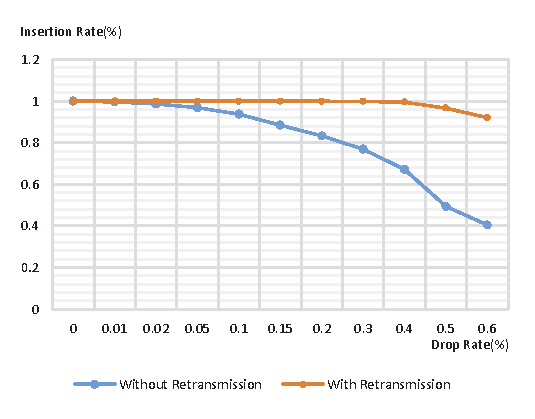
\includegraphics[width=0.7\textwidth]{drop-rate}
  \caption{不同丢包率情况下的数据插入成功率}
  \label{fig:drop-rate}
\end{figure}

\section{存储服务设计原则总结}
NDN Repo对外提供了远程的数据操作服务,并在Repo操作协议中定义了交换的文档格式,信息语义以及交互流程,具备了提供service的基本特征。根据web service的WSMF模型的八要素:Repo的协议已经具备如下要素:

\begin{itemize}
\item 文档类型(Document Types):确定协议间到底采用的是插入协议还是删除协议。
\item 语义(semantics):采用与NDN协议中相似的数据类型,例如:NAME-COMPONENT-TYPE。
\item 相关传输协议:采用NDN作为底层的传输协议。
\item 信息交换序列:完整的数据对象被底层NDN网络分段时,在分段数据包名字后加入了段序号。
\item 流程:无论是插入还是删除的协议都定义了相对完备的流程,在流程中出现的各种状态,都定义了repo的相应操作。
\item 安全:下层的NDN网络定义了针对数据包的基本安全,而在repo协议中对命令请求也进行了证书签名。
\item 句法:采用了TLV格式,同样具备动态伸缩的文档格式。此外由于在TLV格式中包含了数据的长度信息,文档编码解码的效率更高。
\item 服务配置:在repo-ng的实现过程中,repo-ng的配置文件采用了json格式,同时语义比较接近validconf。
\end{itemize}

由上可得,以NDN Repo协议为基础的NDN网络上的服务具备WSMF模型所要求的Web服务的基本要素,可以以repo协议为原型,提出一套基于命名数据网络的服务架构。而相比于Web Service的经典三要素:SOAP,UDDI以及WSDL,目前在基础设计上还是缺位的。具体体现在,虽然在Repo协议中定义了一些命令的消息格式,但是没有一套通用的命令格式。在NDN Packet Specification中,对TLV结构的格式有一套基本定义,但是还没有对命令及其参数等信息的文档描述。最后,在Web Service中UDDI为Web Service功能集成的典型目录系统,虽然NDN协议未必需要一个集成的服务目录,但是需要一套Service Descovery。进一步的为了服务流程自动化,NDN服务协议也需要一套类比于BPEL的服务集成方式。

%%% Local Variables: 
%%% mode: latex
%%% TeX-master: t
%%% End: 

\chapter{命名服务网络设计}
在\ref{SCN-intro}中介绍了集中以信息中心网络为基础的服务网络设计,以上设计方向主要分为两类:
\begin{itemize}
\item 利用服务来对网络连接进行抽象以提高在网络层面的网络服务质量:典型的如SOFIA\cite{wu2014sofia}网络,将命名数据包进一步抽象成命名服务包并对服务转发进行控制。而SERVAL\cite{nordstrom2012serval}网络中,虽然不是直接以ICN为原型,但是通过服务名对数据包进行抽象以达到对网络流量更好的控制。
\item 另一种通过对服务进行抽象以实现功能性网络:典型的如Service Centric Networking\cite{braun2011service}中,通过将数据请求重新封装为服务命令请求,以实现远程调用。在Named Function Networking\cite{tschudin2014named}中不仅以数据处理为核心定义了数据处理请求,同时重新设计了NFD的流程,添加了主动的数据处理整合表达式($\lambda$表达式)。
\end{itemize}

本文旨在通过基于ICN的性质,在网络层面集成网络服务功能,来探索在命名数据基础上进行服务抽象的网络的新的特性。W3C的web service标准参考了WSMF的模型,WSMF模型同样需要基于一些基本要素包括:文档类型,语义,相关传输协议,信息交换序列,流程,安全,句法以及服务配置。文章\cite{pautasso2008restful}中提供了一套比较RESTful Service与Web Service的框架。该框架更加详细地分析了两种web服务在架构设计方面的选择原因。在以往的研究中基于信心中心网络的服务首先没有对服务的前提条件进行研究,同时也没有一套对于服务的基本建模。本节旨在首先结合现有的服务分析框架提出在ICN之上做服务网络的架构选择,提出服务模型,并总结一套设计原则。基于该服务模型,开发命名服务网络原型并进行实验评估。

\section{命名服务网络设计原则}
在第\ref{repo}章中,介绍了NDN Repo协议。本文提出的命名服务网络(Named Service Networking,NSN)以NDN Repo协议设计为蓝本来进行设计。本节采用文献\cite{pautasso2008restful}中的分析框架,对命名服务网络架构在设计上的选择进行分析。

\subsection{设计原则比较}
基于NDN Repo协议以及repo-ng的实现,同Restful Service与Web Service在架构原则上进行比较。

Rest架构利用HTTP动词作为接口的动词,将HTTP协议作为应用的一部分。而WS-*的SOAP协议中HTTP只是Web Service的文档传输协议。Repo协议的实现过程中,采用了类似于Rest的实现方式,将服务请求的语义与NDN的interest结合,即在interest的请求中封装服务请求参数。

Restful Web架构为典型的客户端服务器架构,通过HTTP协议将客户端,浏览器,服务器等连接起来。Rest的异构性通常来自不同的浏览器生产商对HTTP协议的解析渲染的不同。SOAP和WS-*起源于异构性更强更加服务的自治域,甚至可以集成Web出现之前典型的COBOL程序,或者COBRA架构的系统。在WSMF模型中,一个服务的基本要素为:文档类型,语义,传输协议,信息交换序列,流程,安全,句法,服务配置,这8个元素都可以造成客户端与服务端或者服务端之间产生异构性。NSN架构需要解决的第一个主要问题就是\textbf{基本服务要素之间的异构性}。

在松耦合方面,无论是Rest,WS-*以及NSN都与地点解耦。WS-*架构同时具备高可用性,在网络中断或者服务端宕机时,WS-*客户端可以将请求放进队列。而REST架构为远程RPC模式,更倾向为同步调用。在Repo协议中,无论是插入还是删除流程,都定义了在插入不成功的情况下,重传,或者遇到错误返回的情况,更加倾向于RPC模式。但是在repo-ng的具体实现过程中,客户端可以在本地实现队列结构,未被满足的请求可以定期的进行重试。

在服务扩展方面,NSN采用了TLV格式,为典型的树桩结构文档,可以对服务功能进行扩展。


\begin{table}[h]
\centering
\caption{设计原则比较}
\label{tab:arc-principle-comparison}
\begin{tabular}{l|lll}
架构设计原则 & REST & WS-* & NSN \\ \hline \hline
协议层次 & yes & yes & yes \\ \hline
HTTP作为应用层协议 & \checkmark &  &  \\
HTTP作为下层传输协议 &  & \checkmark &  \\
NDN作为应用传输协议 &  &  & \checkmark \\ \hline \hline
异构性处理 & yes & yes & yes \\ \hline
浏览器之间 & \checkmark &  &  \\
企业级中间件 &  & \checkmark &  \\
需要研究 &  &  & ? \\ \hline \hline
松耦合 & yes & yes & yes \\ \hline
可用性(时间) &  & \checkmark & ? \\
位置 & \checkmark & \checkmark & \checkmark \\
服务扩展: &  &  &  \\
统一接口 & \checkmark &  &  \\
XML可扩展 & \checkmark &\checkmark  &  \\
TLV可扩展 &  &  & \checkmark \\ \hline \hline
\end{tabular}
\end{table}

\subsection{概念比较}

WS-*有远程调用以及消息集成两种方式。\cite{vinoski2002putting}而消息集成的方式更加适合松耦合系统的集成。在Repo Protocol中,采用的是远程调用(RPC)的集成方式。在NSN设计,需要定义的第二个问题是\textbf{如何以消息形式集成异构系统}。

在WS-*实现过程中,WSDL作为对服务的描述,另一方面可以看做服务的契约(contract)。在WS-*实现中,有contract-first和contract-last两种方式。REST架构没有一种描述文档,所以为contract-less。在Repo协议以及NDN packet specification中,对TLV文档有描述文档,可以在TLV描述文档基础上定义类似于WSDL的NSN服务描述文档。

Restful架构本质上是对URI所代表的资源进行状态转移。而WS-*是面向服务对象。在Repo协议中,利用URI名字的前缀代表需要操作的对象,通过URI后面封装的文档来对服务进行操作,是一种介于Rest和WS-*之间的模式。

同Restful架构一样,NSN架构需要对资源描述URI设计采用一种漂亮的方法。需要保证URI的持久性,简洁性,可读性,具体化(倾向使用名词),一致性以及抽象性(不要暴漏实现细节)。

在NDN协议中,数据采用TLV的格式进行封装。在NDN repo协议中,定义了一套描述协议报文格式的TLV描述。该描述虽然定义了请求的基本语义,但是没有一套类似于WSDL对于请求响应过程等描述。在NSN设计中,需要定义的第三个问题为\textbf{如何对NSN服务进行描述}。

\begin{table}[h]
\centering
\caption{概念比较}
\label{tab:arc-conceptual-comparison}
\begin{tabular}{l|lll}
架构设计概念 & REST & WS-* & NSN \\ \hline \hline
集成方式 & 1AA & 2AAs & ?AA \\ \hline
远程调用(RPC) & \checkmark  & \checkmark & \checkmark \\
消息 &  & \checkmark & ? \\ \hline \hline
契约设计 & 1AA & 2AAs & ?AA \\ \hline
Contract-first &  & \checkmark & ? \\
Contract-last &  & \checkmark & ? \\
Contract-less & \checkmark &  & ? \\ \hline \hline
服务标注 & 1AA & n/a & ?AA \\ \hline
自己实现 & \checkmark &  & ? \\ \hline \hline
URI设计 & 2AAs & n/a & 2AAs \\ \hline
“Nice” URI scheme & \checkmark  &  & \checkmark \\
No URI scheme & \checkmark &  & \checkmark \\ \hline \hline
数据表述方式 & yes & yes & yes \\ \hline
XML schema &  & \checkmark & ? \\
TLV schema &  & & \checkmark \\
自定义 & \checkmark &  & \\ \hline \hline
\end{tabular}
\end{table}

\subsection{技术比较}
本节讨论在服务网络实现中,在安全性,可靠性,服务集成以及服务发现的架构选择。

\begin{table}[h]
\centering
\caption{技术比较}
\label{tab:arc-tech-comparison}
\begin{tabular}{l|lll}
架构选择 & REST & WS-* & NSN \\ \hline \hline
安全 & 1AA & 1AA & 1AA \\ \hline
WS-Security &  & \checkmark & \\
HTTPS & \checkmark &  & \\
NDN-Security &  &  & \checkmark \\ \hline \hline
传输可靠性 & 1AA & 4AAs & ?AA \\ \hline
HTTPR & (\checkmark)  & (\checkmark) & \\
WS-Reliability &   & \checkmark & \\
WS-ReliableMessaging &   & \checkmark &  \\
Naive &  & \checkmark &  \\
自定义 &  & \checkmark & ? \\ \hline \hline
服务集成 & 2AAs & 2AAs & ?AA \\ \hline
WS-AT &  & \checkmark & ? \\
自定义 & \checkmark & \checkmark & ? \\ \hline \hline
服务集成 & 2AAs & 2AAs & ?AA \\ \hline
BPEL &  & \checkmark & ? \\
Mashups & \checkmark &  & ? \\
自定义 & \checkmark & \checkmark & ? \\ \hline \hline
服务发现 & 1AA & 1AA & ?AA \\ \hline
UDDI &  & \checkmark & ? \\
自己实现 & \checkmark &  & ? \\ \hline \hline
\end{tabular}
\end{table}

WS-*的服务安全采用WS-Security协议\cite{atkinson2002web},而REST安全通常是基于HTTPS提供信任保证。HTTPS的安全模型相对简单,提供的只是点对点的加密以及签名,无法解决跨信任域的安全策略以及信任模型。WS-Security利用现有的相对成熟安全标准与规范来实现,利用X.509和Kerberos进行签名以及身份验证,密钥管理可以基于KPI。由于SOAP协议是基于XML文档进行传输的,采用对XML文档进行加密或签名,在XML的子文档头中封装签名信息。NDN的安全策略与WS-Security类似采用基于文档的安全方式,证书信息封装在NDN命名数据包中。NDN没有指定特定的安全模型,安全策略与信任模型的设计同数据安全通道设计分离。NSN在NDN的基础上采用interest与data双向的安全通道策略。

在WS与REST的工业实现中,数据的可靠传输依靠TCP或TCP类似的可靠传输协议。RESTful作为一种服务实现风格,没有HTTP之上的可靠传输处理流程。WS-*目前有WS-ReliableMessaging\cite{ferris2005web}和WS-Reliability\cite{iwasa2004ws}两种标准。架构基本思路为通过将不可靠基础设施的服务消息传输借道可靠传输通道。在Repo协议中,可以看到对于传输的控制只是对传输正确性的控制,而不是对报文可靠传输真正的控制。NDN并没有对通信有可靠传输保证,NACK也并没有加入到现在的NDN协议之中。作为NSN的扩展,NSN设计的第四个问题为\textbf{如何进行可靠传输协议设计}。

在传输可靠性基础之上就是服务可靠性,即对事务的支持。在WS中提供了对于原子性事务的支持WS-AT。对于分布式事务的支持即为服务集成的基础。

在服务集成上,REST架构没有一个统一集成的标准,在某些领域有通过REST通信方式集成资源的专门协议,如OAuth来解决第三方网站之间信任与认证的问题\cite{hardt2012oauth}。对于Web Service服务集成的研究相对比较成熟,最典型的以BPEL为基础的服务流程集成系统。NSN系统如果想进行功能可扩展同样需要对服务集成的支持。NSN设计的第五个问题为\textbf{如何设计NSN服务描述以支持服务集成},其中包括对于事务扩展以及集成状态触发的支持。

\section{命名服务网络协议概述}
在\cite{braun2013service}中,提出了一种基于ICN的服务网络架构,包括服务解析,服务参数与类型支持等。然而,仅仅拥有这些因素还是无法构建一个分布可用的服务网络。在\cite{fensel2002web}中,提出了一种基于Web Service的服务模型。WSMF模型在\ref{WSMF-arc}中已经进行了介绍,指出了一个可用服务的要素,包括文档类型,语义,传输协议,信息交换序列,流程,安全,语法以及服务配置。

\textbf{服务描述}机制并没有在SCN中阐述。\cite{braun2013service}尽管在SCN中服务请求可以封装命令及相关参数,但在没有服务描述的情况下,客户端与服务端的设计无法做到松耦合。在Web Service中,WSDL用来让web应用去“懂得”如何调用某服务。

\textbf{服务发现}在大型可扩展的网络同样必不可少。Web Service中通过UDDI来管理服务描述文档,并对服务进行简要描述。同样在Web Service基础上有一些街自动服务发现的相关研究。\cite{klusch2006automated,schmidt2004peer,schlosser2002scalable}

\textbf{服务协调}意义在于协调不同的服务语义使服务之间能够以更加可扩展的方式进行沟通。在服务升级过程中,服务语义之间会发生不同版本共存的情况。语义网的本体论技术可以在不同语境下去融合不同的语义术语。

在\cite{braun2011service, braun2013service}中,提出的基于CCN网络的SCN框架可以归纳如下:

\begin{enumerate}[a]
\item 命名:利用$\left\langle content\_owner, content\_name\right\rangle $的命名结构来整合结构化与扁平化命名
\item 服务解析:服务名字与服务地址的匹配
\item 服务参数:在服务与网络耦合的网络中,修改各种ICN网络中内容请求的格式,将请求服务参数放置于内容请求中,如CCN网络;在服务与网络解耦的设计中丰富服务描述系统,如PURSUIT网络
\item 服务部署:通过向服务开发者提供网络环境参数,以优化服务部署方案
\end{enumerate}

但是上面a - d四点无法提供基于ICN的可扩展服务。基于Web Service中的WSMF模型\cite{fensel2002web},提出基于NDN的NSN设计的基本原则:

\begin{enumerate}[a]
\item 在NDN基础上的应用层进行服务网络设计
\item 修改服务请求使服务请求可以被安全验证
\item 可扩展的服务语义与服务描述
\item 建立可扩展的服务解析与发现系统
\item 相似语义的服务可以被协调
\end{enumerate}

基于NDN网络的NSN概念设计如图\ref{fig:NSN-arc}所示,对于NDN网络,NSN层面需要在NDN层面上进行定制化的改动,例如修改Interest名字的结构。

\begin{figure}[H]
  \centering
  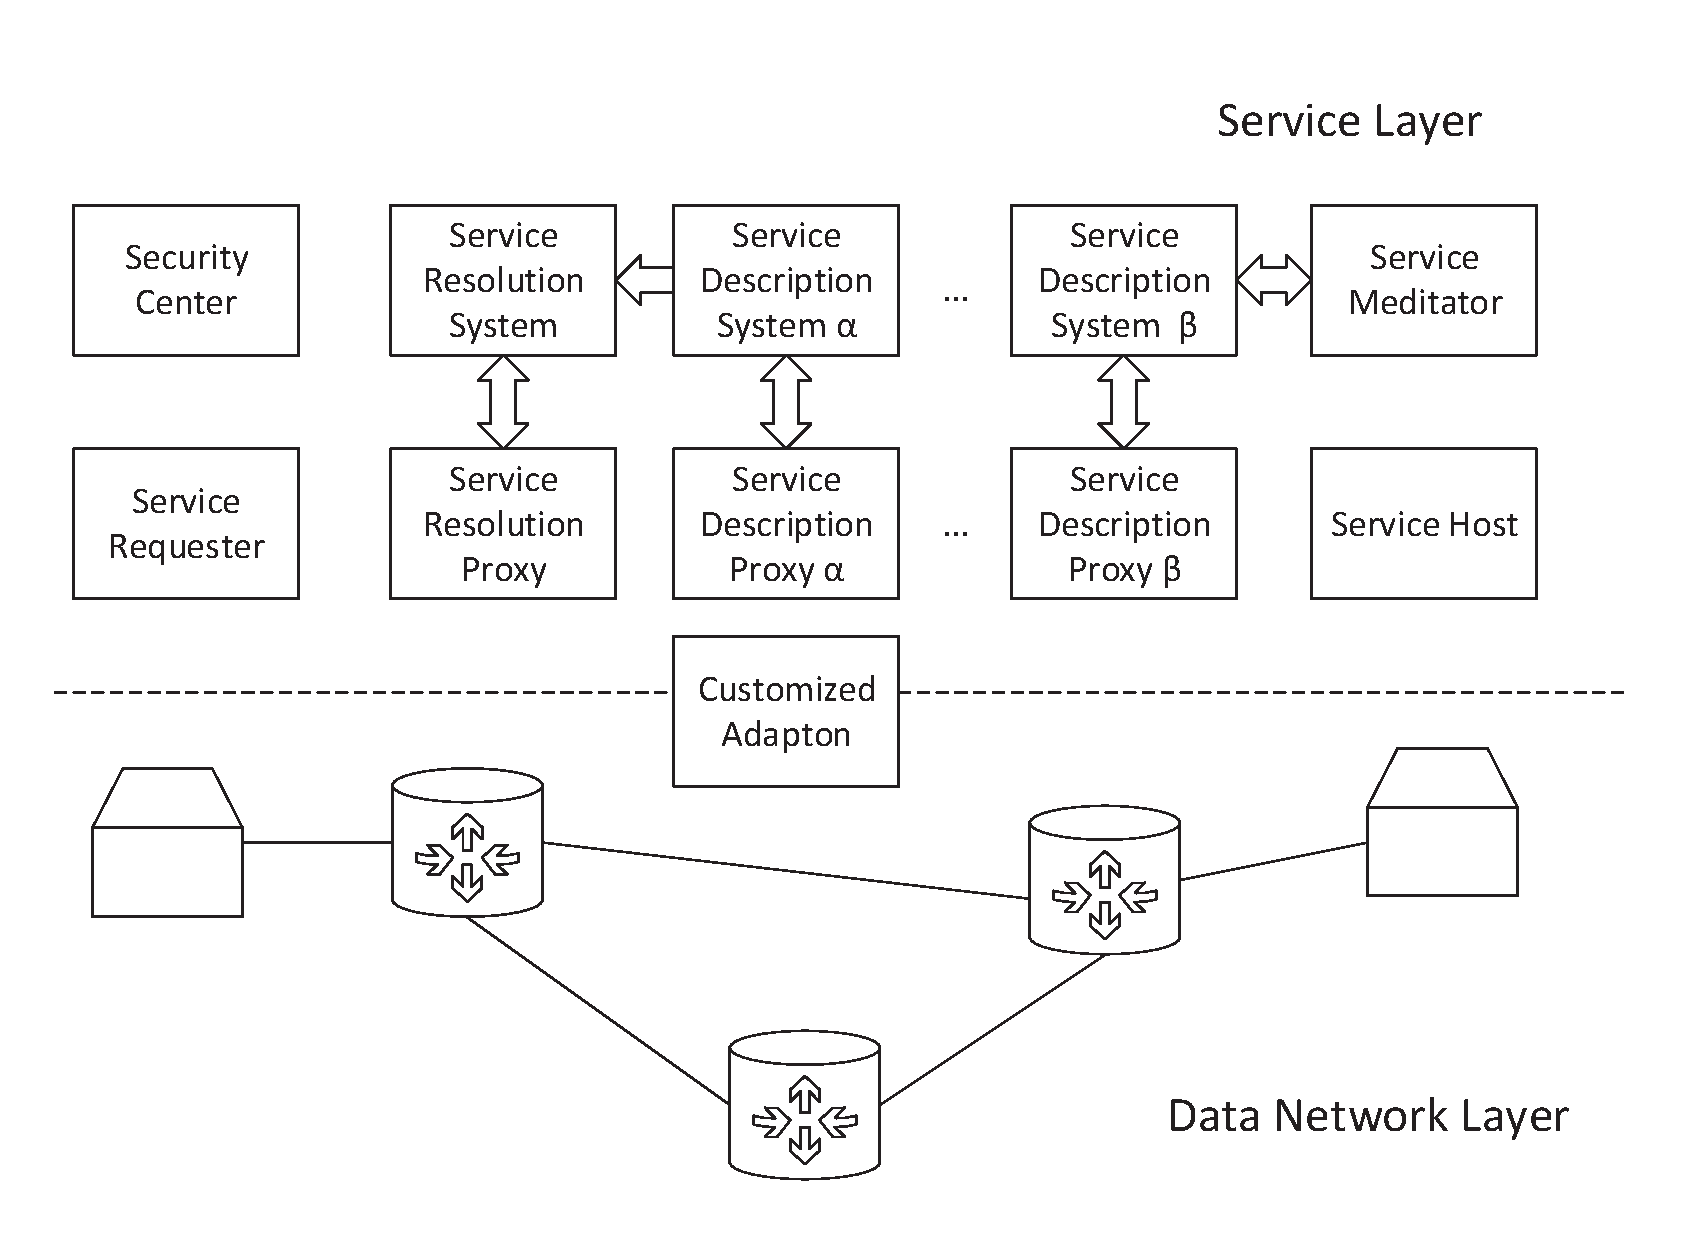
\includegraphics[width=0.8\textwidth]{NSN-ICN}
  \caption{NSN概念架构设计}
  \label{fig:NSN-arc}
\end{figure}

\subsection{服务抽象}
在ICN网络中,网络的作用对命名数据请求响应对应的命名数据。在命名服务网络(NSN)中,网络的目的是用来传输指定的命名服务请求,对该请求进行响应处理并对服务请求者返回请求结果。NSN利用NDN作为下层数据传输协议,采用类似于RESTful方式,将服务请求封装在NDN数据请求之中,NDN数据包封装服务响应。NSN并没有修改下层NDN协议,包括网络包封装协议,路由协议等。NSN可以被看做基于NDN的一种分布式应用服务。在NSN中,服务请求是服务的触发条件,服务的标识为服务的名字,采用NDN URI的命名惯例。服务描述以TLV描述文档为基础,构建类WSDL的文档描述协议。

\subsection{安全}
安全性为服务网络可用性的基础。服务安全性最基础的要求为,服务请求与响应可被验证与加密。除此之外需要服务请求与响应所绑定的安全身份可以被公开验证。服务请求所绑定的安全身份可以被用来进行服务访问控制。

NDN采用基于内容/文档的安全机制。所有的数据包采用密钥进行数字签名,证书信息被封装在数据包之中。在原始的NDN协议中,并没有对数据请求签名的支持。在NSN中,采用在NDN静态库ndn-cxx中SignedInterest\footnote{Signed Interest: http://named-data.net/doc/ndn-cxx/0.3.1/tutorials/signed-interest.html}的实现。

NSN的双向签名网络包是实现安全的基本保证。在NSN设计中,上层具体的安全构建并没有作为强制标准,在NSN实现中采用安全中心设计。在当前的签名与加密实现中,工业界普遍采用对称/非对称密钥方式,如Kerberos或X.509。在对称密钥体系如Kerberos中,需要Kerberos认证服务器(AS)作为证书管理与信任锚点(trust anchor)。在非对称密钥体系中,需要公钥基础设施(PKI)对证书与密钥进行管理,需要trust anchor对于证书身份进行验证。无论是何种安全体系,都需要一个相对集中的安全管理角色。在NSN架构实现中,该角色为安全中心。NSN安全中心不是特指具体某一个主机,可以为架构或p2p层次的主机群。

\subsection{服务解析}
在SCN中,服务解析指的是服务寻址。对于通过服务一般描述来获取服务描述文档,单纯的名字寻址无法满足要求。当前通过服务描述来获得具体服务文档的话有如下几种方式:

本体论:例如在语义网实现的Web Service实现中,OWLS-MX提供了一种基于本体论的具有语义推导功能的服务发现协议。\cite{klusch2006automated}

分布式查询系统:分布式查询系统可以将服务发现服务进行分布式布置,利于系统服务的扩展。典型系统如基于本题论的Hypercube P2P系统\cite{schlosser2002scalable},以及基于分布式哈希的关键词查询系统\cite{schmidt2004peer}。

WS-*工业一般实现中采用UDDI的集中式注册目录作为服务发现系统。在NSN设计中,采用服务解析代理作为服务请求者服务解析入口。NSN服务解析层次作为独立的系统接收服务解析代理的查询请求。在实际系统实现中,NSN采用关键词搜索方案。当前互联网解析服务中,本体论应用场景比较少。随着搜索引擎技术的发展,关键词匹配的技术效果越来越好,同时采用关键词方法的学习成本相对较小。同时有一些方便的开源项目例如Apache Lucene\footnote{Apache Lucene: https://lucene.apache.org/core/}提供了非常方便的文档关键词查询的解决方案。

服务解析代理需要预先定义好服务解析的语义,并了解服务解析主机的名字。服务解析代理只是负责发送服务解析请求,并需要了解服务解析主机服务的部署方式,无论是中心化,层次化还是P2P的。

\subsection{服务描述}
\label{description}
对于一个服务描述需要包含以下六个元素:
\begin{enumerate}[a]
\item 服务的名字
\item 服务描述与关键词:用来在文本上描述服务,并为服务发现提供索引依据。
\item 功能列表:该服务可以提供功能的名字列表
\item 先决条件(Pre-condtions):触发服务某功能需要的先决条件,通常情况下为输入参数。此外,对于支持状态的服务,同样包含触发服务需要的状态。
\item 输出条件(Post-conditions):描述在不同状态下服务的返回条件。通常为返回值参数描述。在状态服务下,同样会输出服务状态的变化。
\item 服务拥有者。
\end{enumerate}

一个典型的服务描述如下所示,该服务描述描述了一种数据存储服务。该服务基本功能参照NDN Repo协议,通过普通的NDN interest来获取数据,数据插入与删除作为服务功能开放。该描述用伪代码部分展示如后框图所示。WSDL中,对于服务的描述以XML形式进行封装。虽然在概念设计上,NSN服务描述没有规定指定的文档格式。在实现中则采用TLV结构的可扩展的文档结构。服务代理当有服务的确切名字时,可以利用该名字发送interest,请求服务描述数据包。服务描述系统将服务描述数据包返回给服务代理。而根据关键词以及部分文档描述进行查询则被当做服务描述系统的一种服务对外开放,接收的是服务请求而不是单纯的数据请求。

Web Service中WSDL设计的要素包括:definitions,types,portType,operation,binding,service以及port。在NSN中,由于专门binding在NDN上,operation可以作为名字的一部分封装在服务请求中,并与服务描述中的function list的名字进行一一对应。此外在TLV文档描述中,描述了输入参数的类型,对应于WSDL中的Type。WSDL中definitions即作用域可以用名字的前缀来进行对应。在形式上WSDL与NSN的文档描述可以进行等价。

\begin{figure}[h]
\begin{framed}
\begin{verbatim}
Repo Service Description

Name: /THU/repo
Description: insertion and deletion of data packets
Keywords: repository, repo, insertion, deletion, removal,
          data packet
Function List:
    Name: insert
        Description: put data packets into repo
    Name: delete
        Description: remove data packets from repo
PreCondition:
    FunctionName: insert
        Parameter: DataName
            DataName: BYTE
    FunctionName: delete
        Parameter: DataName
            DataName: BYTE
PostCondition:
    FunctionName: insert
        Result: StatusCode
        StatusCode: INTEGER
    FunctionName: delete
        Result: StatusCode
\end{verbatim}
\end{framed}
\end{figure}

\subsection{服务协调与集成}
在前述服务描述文档结构中,为服务集成提供了输入与输出状态描述。在Web Service服务集成中,分别有Orchestration和Choreography两种模式。考虑到NSN对于服务的描述与WSDL在形式上可以进行等价。对于BPEL的设计经验同样可以移植在设计NSN的服务集成当中。

除了服务集成之外,还有就是语义协调。文档的设计上可以分为兼容关系与匹配关系两种,对于服务描述文档的兼容或匹配的判断可以交给NSN中专门的协调单元。

在图\ref{fig:NSN-arc}中,mediation模块抽象的代表了服务集成引擎(类比于BPEL engine)以及服务语义协调的功能。

\section{命名服务网络原型实现}
命名服务网络NSN原型基于NDN的开源代码库,包括ndn-cxx,NFD以及NLSR。通过修改ndn-cxx基础库,增加对于NSN服务描述的支持。NSN原型实现了三种服务,包括空服务,即服务端只返回一个空内容的服务返回包;基于NDN Repo协议的存储服务;提供简单四则运算的计算服务。本节将分别介绍各个要素的实现。原型实现代码已经在Github上开源:https://github.com/chenatu/repo-service

\subsection{命名}
服务请求的命名方式采用NDN的模块化URL。在当前的NDN网络包中,采用TLV的封装格式,TLV可以通过子模块组合而成。在NDN命名中,数据请求的名字为完整的TLV模块,通过每个子名字单元TLV模块组合而成。而每个子单元可以由更加小的TLV模块组合而成,由此可以封装服务请求的参数。服务请求的名字结构如下所示:
\begin{framed}
\begin{verbatim}
/service name/function name/parameter
\end{verbatim}
\end{framed}
其中function name模块为服务描述function list中服务功能名字。parameter结构可以对参数进行结构化封装。以数据插入请求为例,参数的TLV结构为:
\begin{framed}
\begin{verbatim}
Parameter ::= REPOCOMMANDPARAMETER-TYPE TLV-LENGTH
                           Name?
                           Selectors?
                           StartBlockId?
                           EndBlockId?
                           ProcessId?
                           MaxInterestNum?
                           WatchTimeout?
                           WatchStatus?
                           InterestLifetime?
\end{verbatim}
\end{framed}

其中Parameter可以由包括Name,Selectors在内的子结构组成。

\subsection{安全}
NSN的安全设计采用NDN Repo协议中的基本安全设计。采用Signed Interest与Signed Data Packet的方式为服务请求与服务响应验证。服务签名,时间戳,以及为了避免重复的随机值作为名字子结构增加在服务请求名字之后。
\begin{framed}
\begin{verbatim}
/service name/function name/parameter/signature/timestamp
/random-value
\end{verbatim}
\end{framed}

在NSN设计中的安全中心,在本NSN的原型中主要作用为:构建信任锚点(trust anchor)以及保存身份公钥。安全中心系统以\textit{repo-ng}实现。

\subsection{语义}
NSN的服务描述设计遵循\ref{description}中服务描述的设计。服务描述文档同样以TLV格式进行封装。在Web Service语义与实现的对应中,有before-contract以及post-contract的模式。在NSN存储服务的设计中采用了post-contract的模式,即先设计服务描述文档,根据描述实现功能代码。但是在广域服务网络中,出于开发的分布性,对于同样的名字服务会开发出不同的服务描述,由此产生不同的语义。在实现中,通过repo-ng作为语义描述的后台存储,将语义描述封装进NDN数据包之中。对于同名的不同语义,通过PublicKeyLocator来对描述发布者来进行区分。

\subsection{服务发现}
服务发现实现采用了Apache Lucence系统,并开发了服务查询服务。服务描述管理机群与服务代理开放相同的服务描述语义,通过不同的命名空间加以区分。服务代理通过接收服务查询请求,将服务查询转发给服务描述管理机群,并对服务描述进行本地缓存。当服务请求端再次请求相同请求时,可以利用缓存进行响应。服务查询语义中采用query-service作为查询动词。服务查询参数结构如下所示。通过服务名前缀,关键词,描述等匹配。Selector中可以为返回数据包增加限制条件,其中比较重要的是通过PublicKeyLocator选择子对服务的所有者进行限定。

\begin{framed}
\begin{verbatim}
Parameter ::= QUERYPARAMETER-TYPE TLV-LENGTH
                           Name?
                           Keyword?
                           Description?
                           Selector?
\end{verbatim}
\end{framed}

\subsection{服务集成与协调}
在本工作中,NSN原型只是形成了功能上的服务集成,并没有开发类似于BPEL类的服务集成语言。服务集成是通过在Mediator中开放指定的集成类型服务,定义服务描述模板,并在代码中实现该集成功能。本工作中实现了简单的加减法四则运算式功能。计算服务可以处理单独的加法或减法。如果是混合加减法则需要将服务请求发给Mediator中,Mediator通过解析服务请求参数来分别调用加法服务与减法服务,从而实现了简单的运算请求。

NSN原型解决的另一个服务协调的问题为,当服务描述过期,更新版本时导致服务请求无法被正确识别是。可以向Mediator发送语义过时的服务请求,Mediaotor会将该请求翻译为更新的服务请求。目前实现的为当参数扩充时,服务请求的重构。

\section{实验评估}
实验平台采用Amazon Web Service提供的虚拟机服务。采用虚拟机配置为m3.large。在该配置下vCPU 2个,ECU为6.5,7.5G内存,32GB的SSD存储。在文献\cite{wang2010impact}中分析了Amazon EC2系统虚拟化对网络性能的影响,当采用medium以上的服务配置时,对网络性能影响已经非常小。因此实验采用large级别的服务器配置。

操作系统采用Ubuntu 14.04。实验软件平台采用NDN Forwarding Deamon作为NDN协议转发软件,利用UDP作为下层传输协议。NSN服务端采用以repo-ng为基础的存储服务工具,网络环境为在弗吉尼亚的Amazon数据中心内部。

\subsection{服务传输效率比较}
在当前网络服务中,数据相关服务是重要服务之一,在数据服务中,数据传输效率是影响服务性能的重要指标。为了证明NSN在传输方面的效率,实验比较了基于NSN的repo服务以及基于SOAP协议的repo服务。在基于SOAP协议的repo服务中,采用与repo协议同样的流程。数据包同样采用命名分段传输,即一个命名数据对象以NDN形式进行数据包分段。SOAP协议实现基于gsoap\cite{van2007gsoap}软件包。

图\ref{fig:getfile}表示的是,NSN与SOAP在数据读取服务中的传输效率比较。数据传输为在一个数据中心网络中的两个不同的24位子网掩码之间的两台主机进行点对点传输。数据传输模式为发送一个数据段的数据段请求,repo服务返回对应数据段的命名数据包,同时数据请求发送采用了流水线的模式,流水线大小为20。实验分别比较了当文件大小为1M~1000M文件传输时间对比。从图\ref{fig:getfile},基于SOAP的传输速度要慢于基于NSN传输速度将近10倍。从图中还可以看到,传输速度在不同的文件大小中基本恒定,并且NSN在不同数据包大小的情况下传输速度基本一致

\begin{figure}[H]
  \centering
  \includegraphics[width=0.7\textwidth]{getfile}
  \caption{NSN和SOAP协议下读取数据比较}
  \label{fig:getfile}
\end{figure}

图\ref{fig:putfile}表示的是,NSN与SOAP在repo数据发送插入速率比较。硬件与网络环境与前面实验相同。基于SOAP的数据插入同样采用repo协议的插入流程。实验分别比较了文件大小为1M~1000M文件插入时间对比;基于NSN的插入速度要稍快于基于SOAP的插入速度,约为1.5倍左右。在不同文件大小下,数据插入速度基本一致。


\begin{figure}[H]
  \centering
  \includegraphics[width=0.7\textwidth]{putfile}
  \caption{NSN和SOAP协议下插入数据比较}
  \label{fig:putfile}
\end{figure}

在数据获取实验中我们可以看到,采用NSN作为服务协议,数据传输的效率会提升很多。首先从网络架构角度来说,NSN在NDN路由层面对数据进行路由。而SOAP被HTTP协议所封装,每一次服务请求都要开启一次HTTP连接。每一次HTTP请求,在底层需要进行一次TCP链接开启,即TCP握手,需要经历1.5倍RTT时间,每次请求之前都需要有1.5倍RTT,同时TCP关闭通常也需要2RTT的时间。在AWS us-east-1a区域中,平均RTT为0.263ms,数据传输外的延时约为1ms。因此在针对与大量数据传输服务中,WS-*架构的SOAP协议并不适合。

在数据插入中,我们可以看到相比于数据读取会有一个比较大的速度下降。由于我们底层采用sqlite数据库做存储。Sqlite开发官方在1.6GHz CPU, 1M内存对数据插入与读取进行测试\footnote{Database Speed Comparison: https://www.sqlite.org/speed.html}。1000次插入需要13s,而利用索引查询数据1000次大约为0.22s。两者相差将近50倍,所以插入的性能下降主要由数据库的I/O产生。

与基于HTTP的WS-*架构相比,基于NDN的NSN架构可以充分利用网络中对于命名数据的缓存特性,即发送请求之后,请求结果会在本地进行缓存,对于相同的服务请求可以先利用本地缓存进行响应。在图\ref{fig:cache}的实验中,分别在N. Virginia和Oregon之间发送数据请求NSN与WS请求。图\ref{fig:cache}表示的是其分别在不同数量的相同请求下,服务的总响应时间。可以看到由于SOAP协议并无缓存性质,其请求总时间也是随着请求数量线性增长的。

\begin{figure}[H]
  \centering
  \includegraphics[width=0.7\textwidth]{cache}
  \caption{NSN和SOAP在发送重复请求下的效率对比}
  \label{fig:cache}
\end{figure}

图\ref{fig:cache-2}表示的是就近缓存对服务传输效率提升的影响。实验中,服务端虚拟机在Oregon,在N. Virginia部署4台服务请求端。如图\ref{fig:cache-2}当,第一个NSN服务请求时,请求延时约为0.09ms。其它服务端发送相同的服务请求时,可以从N. Virginia本地缓存的服务请求得到请求响应,平均时间为1ms。

\begin{figure}[H]
  \centering
  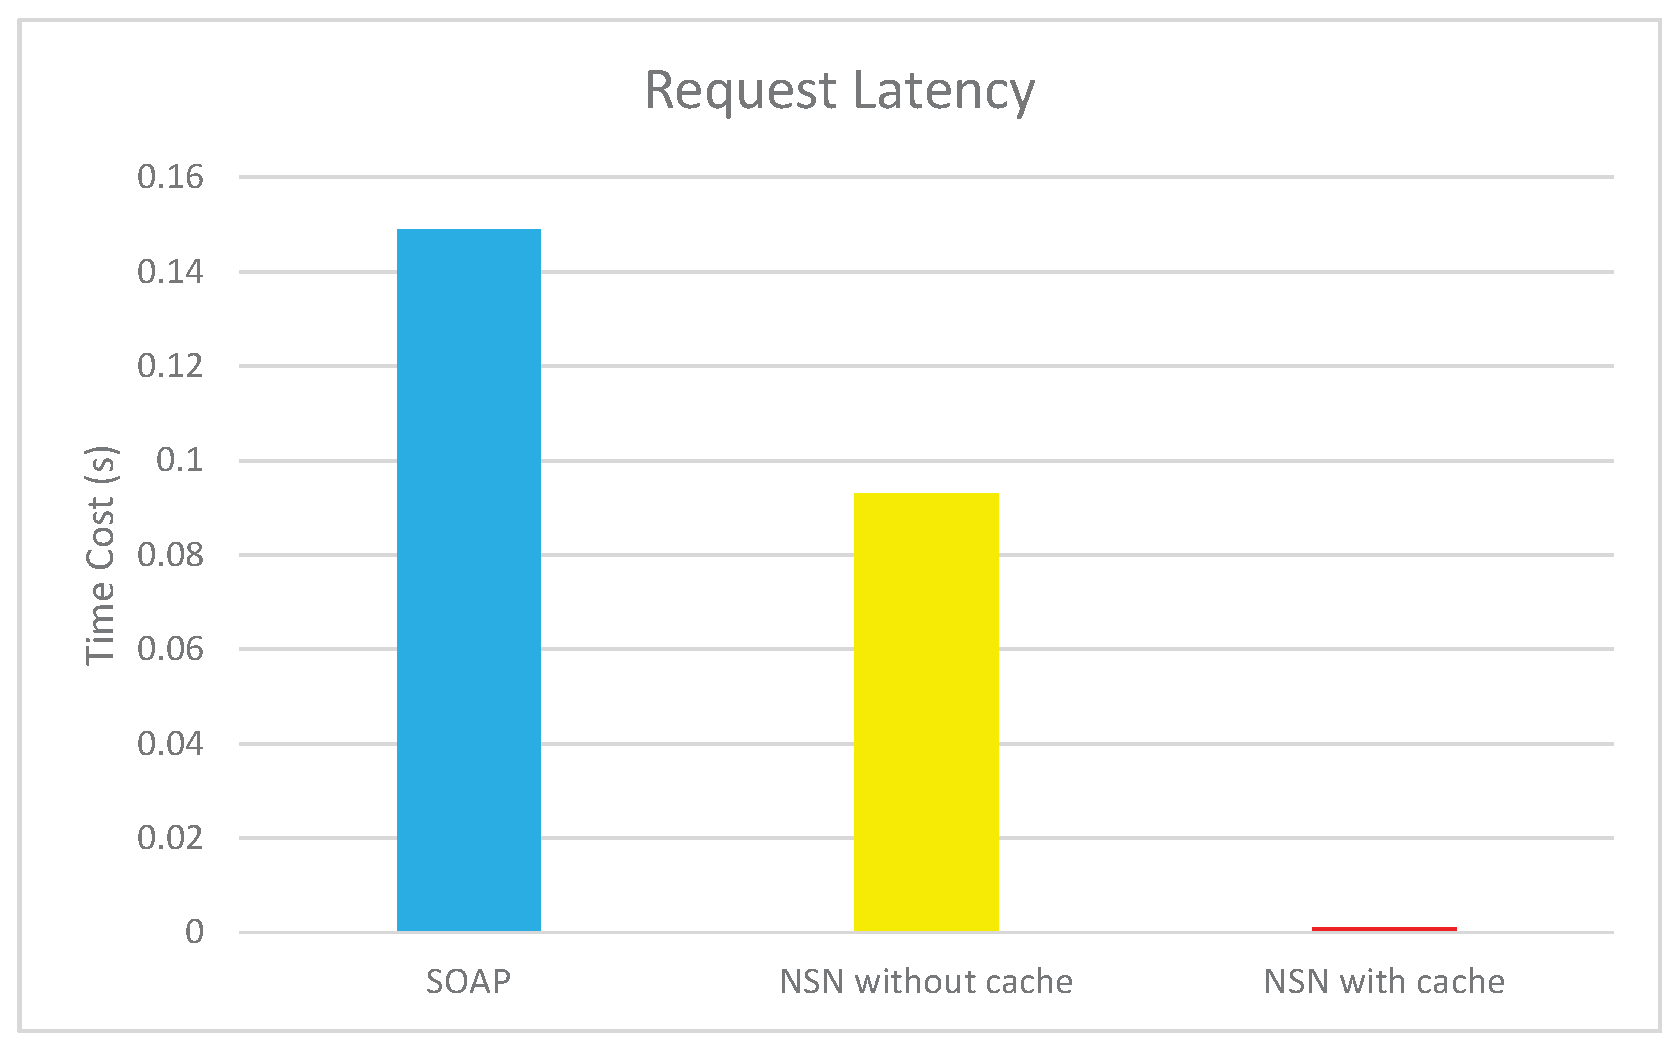
\includegraphics[width=0.7\textwidth]{cache-2}
  \caption{NSN缓存对传输速度的影响}
  \label{fig:cache-2}
\end{figure}

\subsection{服务迁移}
NSN的一个重要特性是将服务的名字与服务的具体位置解耦,服务可以不仅仅限制在同一台主机上。同时由于NSN的安全属性,同名服务还可以在多台主机上同时分布。在云计算服务中,虚拟机或者服务进程迁移在负载均衡以及服务弹性配置中是一项重要功能。本实验评估了服务从一台主机迁移到另一台主机的时候对服务的影响。实验环境为同一数据中心网络的两个子网。客户端在向一台主机不断地请求服务。在10s时服务在一台主机上关闭的同时,在另一台机器上启动。图\ref{fig:migration}表示在实验过程中,客户端发送的请求被响应的情况。可以看到在0.2秒内服务得到恢复。

\begin{figure}[H]
  \centering
  \includegraphics[width=0.7\textwidth]{migration}
  \caption{服务迁移对服务请求处理的影响}
  \label{fig:migration}
\end{figure}

\subsection{服务可用性}
在分布式的服务网络中,服务的可用性也是一项重要的服务评价指标。在本实验中,在N. Virginia的不同子网中部署了四台相同提供相同服务的主机,即服务名字前缀相同。在Oregon数据中心中恒定发送每秒200次服务请求。服务端在0s中启动两台1,2号服务主机,10s时3号服务主机,20s时启动4号服务主机,30是时关闭1号服务主机,40是时关闭2号服务主机,50s时关闭3,4号服务至极服务主机。在图\ref{fig:avail-2}中,可以看到服务请求与服务处理速度基本相等,在40s附近有非常短暂的服务中断。分布式系统中单独服务的频繁启动关闭对于服务可用性的影响很小。

\begin{figure}[H]
  \centering
  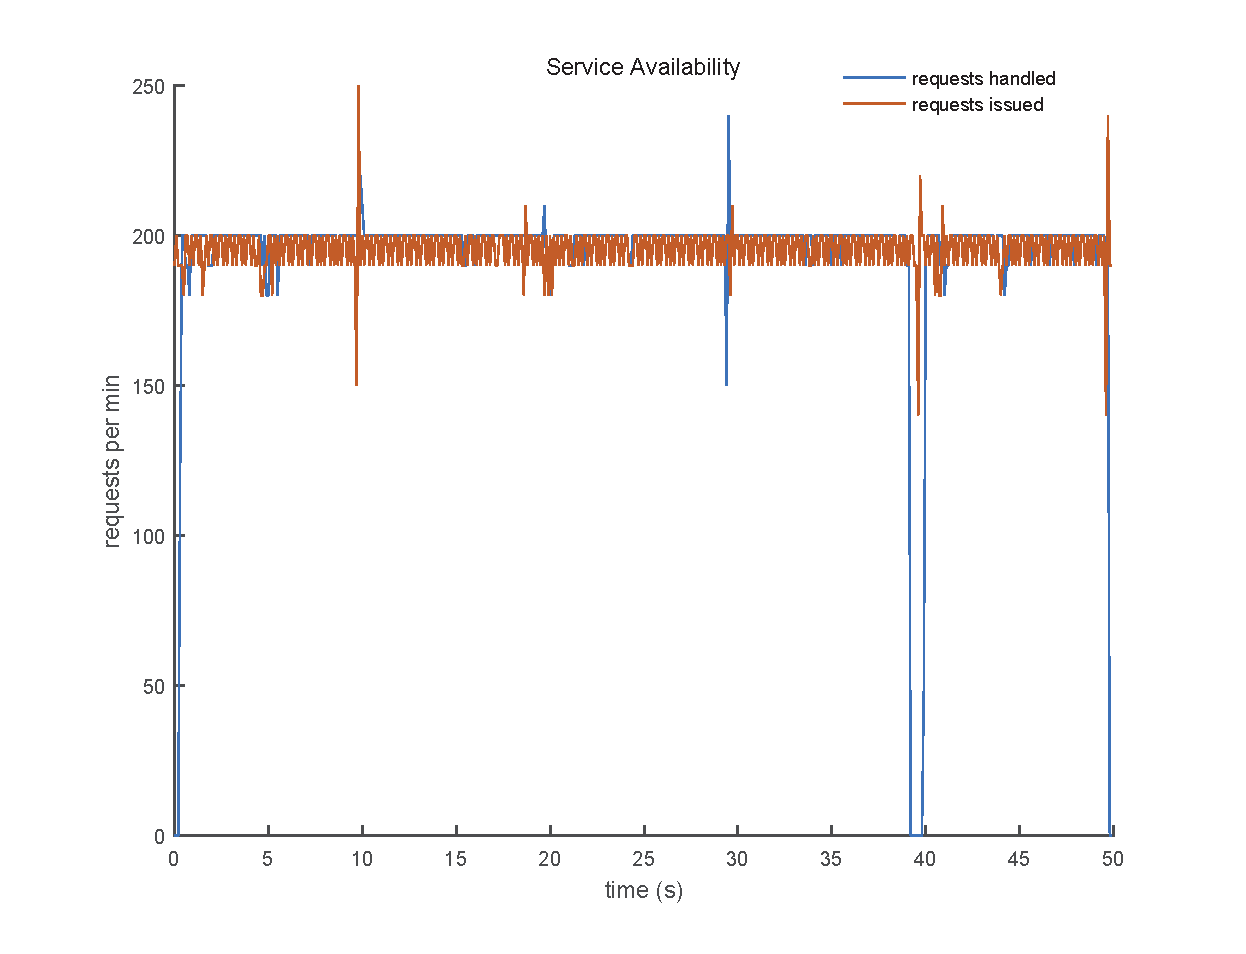
\includegraphics[width=0.7\textwidth]{avail-2}
  \caption{服务可用性测试}
  \label{fig:avail-2}
\end{figure}

\subsection{服务策略配置}
NSN基于NDN网络进行请求的路由和转发。在NDN网络中,可以配置请求转发策略。在本实验中配置了两种转发策略,best-route和随机转发策略。best-route为NDN的默认转发策略,即转发给最近转发请求中,平均延时最小的一个端口。rondom策略为随即平均地转发给任意一个端口。图\ref{fig:strategy:best-route}中表示为在best-route策略下,两台相同服务的主机响应请求的情况。可以看到当网络服务质量比较好时,始终转发到同一个服务主机。图\ref{fig:strategy:random}中表示随机转发策略下两台主机的服务处理情况,可以看到服务响应速率基本一致。

\begin{figure}[H]
\begin{minipage}[t]{0.5\linewidth}
\centering
\includegraphics[width=2.5in]{best-route}
\caption{best-route策略双host请求处理分布}
\label{fig:strategy:best-route}
\end{minipage}%
\begin{minipage}[t]{0.5\linewidth}
\centering
\includegraphics[width=2.5in]{random}
\caption{random策略双host请求处理分布}
\label{fig:strategy:random}
\end{minipage}
\end{figure}

\subsection{服务扩展性}
服务扩展性指的是,服务性能可以随服务主机的增加线性扩展。在本实验中,N. Virginia的不同子网中运行四台服务,服务转发采用random策略,同时客户端以比较大的速率发送服务请求。在0s时启动两台服务主机,并在10s时再启动两台主机。图\ref{fig:scale}表示的是四台服务主机处理请求总和的情况。可以看到在小范围内可以实现服务性能的线性扩展。但是服务性能的扩展性同样受制于转发程序的处理效率,网络带宽等因素,本实验只是在前两者性能得到保证情况下的性能可扩展。

\begin{figure}[H]
  \centering
  \includegraphics[width=0.7\textwidth]{scale}
  \caption{服务扩展测试}
  \label{fig:scale}
\end{figure}

\section{综合分析与结论}


%%% Local Variables: 
%%% mode: latex
%%% TeX-master: t
%%% End: 

\chapter{基于命名数据网络的分布式系统设计}


%%% Local Variables: 
%%% mode: latex
%%% TeX-master: t
%%% End: 

\chapter{总结与展望}

\section{论文工作总结}
本论文主要研究了基于命名数据网络的命名服务网络(Named Data Networking, NSN),及基于命名服务网络的存储服务。研究思路为,首先作者参加NDN社区开源项目设计了基于NDN的数据存储协议NDN Repo,并基于NDN Repo协议开发了数据存储软件repo-ng;以NDN Repo协议为基础,本文提出了一种基于NDN的一般化的服务网络设计框架,与web service,REST架构进行了比较研究。在新的命名服务网络架构基础上,重新规范了存储协议设计;在新的基于命名服务网络的存储协议之上,提出了一种分布式存储架构,以应用层帧设计理念为基础,减少了在网络与本地数据转换,以及网络传输中的冗余。

本文的主要结论与贡献为:
\begin{enumerate}
\item 本文首次提出了一种真正可以远程访问的命名数据网络的数据存储服务。以签名数据请求协议为基础,建立了远程存储主机的可靠访问模式。开发的repo-ng存储软件得到了NDN研究社区的广泛使用。
\item 以命名数据网络为基础,建立了从命名数据到命名服务的抽象。根据WSMF模型,提出了一套在命名服务网络基础上建立服务的设计原则。一方面,基于服务描述文档的服务架构可以提高服务网络的应用扩展性。另一方面,在网络层之上建立服务网络,简化底层网络协议栈,提高服务传输效率。本文对服务网络的扩展性,可用性以及传输效率进行了测试。在中等规模的网络中,NSN的存储服务可以在数据转发的性能瓶颈内进行线性扩展;局域网内服务迁移可以在1 ms左右恢复服务;与Web Service服务相比,提高了网络传输效率。
\item 以命名服务网络以及NDN Repo协议为基础建立了分布式的命名数据存储服务。命名服务网络构建了命名数据存储服务的操作性基础。同时根据应用层帧的设计原则,提出了本地转发数据请求表结构(LFIB)减少了网络数据与本地数据转换的冗余;提出了基于命名服务网络的underlay网络设计,减少了网络传输过程中,复杂网络协议栈的传输冗余。
\end{enumerate}

\section{未来的研究工作}
命名数据网络是一种新的面向数据的网络架构体系,在新体系下,需要特定协议支持上层的应用开发。本文的命名服务网络协议推出了一种支持安全可扩展的一种协议范式。未来可以作为IETF的一种基于NDN的上层协议进行更广泛的合作研究。在命名网络本身,如何构建更加可扩展的服务描述体系,如何更好的进行多服务的集成都是可以深入研究的问题。在应用层面,同样可以基于命名服务网络开发更广泛的服务应用促进研究。

在基于命名服务网络的存储方面,本论文提出LFIB结构以及underlay网络来提高数据处理与传输效率。但是在分布式存储中,数据一致性,服务可用性以及分区容错性都是可以进行深入研究的问题。多个元数据描述表如何协调,多点数据如何同步以及很多经典的分布式存储问题都是命名数据存储今后的研究方向。

%%% 其它部分
\backmatter

% 本科生要这几个索引,研究生不要。选择性留下。
\makeatletter
\ifthu@bachelor
  % 插图索引
  \listoffigures
  % 表格索引
  \listoftables
  % 公式索引
  %\listofequations
\fi
\makeatother


% 参考文献
\bibliographystyle{thubib}
\bibliography{ref/refs}


% 致谢
%%% Local Variables:
%%% mode: latex
%%% TeX-master: "../main"
%%% End:

\begin{ack}
  衷心感谢导师 xxx 教授和物理系 xxx 副教授对本人的精心指导。他们的言传身教将使
  我终生受益。

  在美国麻省理工学院化学系进行九个月的合作研究期间,承蒙 xxx 教授热心指导与帮助,不
  胜感激。感谢 xx 实验室主任 xx 教授,以及实验室全体老师和同学们的热情帮助和支
  持!本课题承蒙国家自然科学基金资助,特此致谢。

  感谢 \thuthesis,它的存在让我的论文写作轻松自在了许多,让我的论文格式规整漂亮了
  许多。
\end{ack}


% 附录
%\begin{appendix}
%%%% Local Variables: 
%%% mode: latex
%%% TeX-master: "../main"
%%% End: 

\chapter{外文资料原文}
\label{cha:engorg}
As one of the most widely used techniques in operations research, {\em
  mathematical programming} is defined as a means of maximizing a quantity known
as {\em objective function}, subject to a set of constraints represented by
equations and inequalities. Some known subtopics of mathematical programming are
linear programming, nonlinear programming, multiobjective programming, goal
programming, dynamic programming, and multilevel programming$^{[1]}$.

It is impossible to cover in a single chapter every concept of mathematical
programming. This chapter introduces only the basic concepts and techniques of
mathematical programming such that readers gain an understanding of them
throughout the book$^{[2,3]}$.


\section{Single-Objective Programming}
The general form of single-objective programming (SOP) is written
as follows,
\begin{equation}\tag*{(123)} % 如果附录中的公式不想让它出现在公式索引中,那就请
                             % 用 \tag*{xxxx}
\left\{\begin{array}{l}
\max \,\,f(x)\\[0.1 cm]
\mbox{subject to:} \\ [0.1 cm]
\qquad g_j(x)\le 0,\quad j=1,2,\cdots,p
\end{array}\right.
\end{equation}
which maximizes a real-valued function $f$ of
$x=(x_1,x_2,\cdots,x_n)$ subject to a set of constraints.

\newtheorem{mpdef}{Definition}[chapter]
\begin{mpdef}
In SOP, we call $x$ a decision vector, and
$x_1,x_2,\cdots,x_n$ decision variables. The function
$f$ is called the objective function. The set
\begin{equation}\tag*{(456)} % 这里同理,其它不再一一指定。
S=\left\{x\in\Re^n\bigm|g_j(x)\le 0,\,j=1,2,\cdots,p\right\}
\end{equation}
is called the feasible set. An element $x$ in $S$ is called a
feasible solution.
\end{mpdef}

\newtheorem{mpdefop}[mpdef]{Definition}
\begin{mpdefop}
A feasible solution $x^*$ is called the optimal
solution of SOP if and only if
\begin{equation}
f(x^*)\ge f(x)
\end{equation}
for any feasible solution $x$.
\end{mpdefop}

One of the outstanding contributions to mathematical programming was known as
the Kuhn-Tucker conditions\ref{eq:ktc}. In order to introduce them, let us give
some definitions. An inequality constraint $g_j(x)\le 0$ is said to be active at
a point $x^*$ if $g_j(x^*)=0$. A point $x^*$ satisfying $g_j(x^*)\le 0$ is said
to be regular if the gradient vectors $\nabla g_j(x)$ of all active constraints
are linearly independent.

Let $x^*$ be a regular point of the constraints of SOP and assume that all the
functions $f(x)$ and $g_j(x),j=1,2,\cdots,p$ are differentiable. If $x^*$ is a
local optimal solution, then there exist Lagrange multipliers
$\lambda_j,j=1,2,\cdots,p$ such that the following Kuhn-Tucker conditions hold,
\begin{equation}
\label{eq:ktc}
\left\{\begin{array}{l}
    \nabla f(x^*)-\sum\limits_{j=1}^p\lambda_j\nabla g_j(x^*)=0\\[0.3cm]
    \lambda_jg_j(x^*)=0,\quad j=1,2,\cdots,p\\[0.2cm]
    \lambda_j\ge 0,\quad j=1,2,\cdots,p.
\end{array}\right.
\end{equation}
If all the functions $f(x)$ and $g_j(x),j=1,2,\cdots,p$ are convex and
differentiable, and the point $x^*$ satisfies the Kuhn-Tucker conditions
(\ref{eq:ktc}), then it has been proved that the point $x^*$ is a global optimal
solution of SOP.

\subsection{Linear Programming} 
\label{sec:lp}

If the functions $f(x),g_j(x),j=1,2,\cdots,p$ are all linear, then SOP is called
a {\em linear programming}.

The feasible set of linear is always convex. A point $x$ is called an extreme
point of convex set $S$ if $x\in S$ and $x$ cannot be expressed as a convex
combination of two points in $S$. It has been shown that the optimal solution to
linear programming corresponds to an extreme point of its feasible set provided
that the feasible set $S$ is bounded. This fact is the basis of the {\em simplex
  algorithm} which was developed by Dantzig as a very efficient method for
solving linear programming.
\begin{table}[ht]
\centering
  \centering
  \caption*{Table~1\hskip1em This is an example for manually numbered table, which
    would not appear in the list of tables}
  \label{tab:badtabular2}
  \begin{tabular}[c]{|c|m{0.8in}|c|c|c|c|c|}\hline
    \multicolumn{2}{|c|}{Network Topology} & \# of nodes & 
    \multicolumn{3}{c|}{\# of clients} & Server \\\hline
    GT-ITM & Waxman Transit-Stub & 600 &
    \multirow{2}{2em}{2\%}& 
    \multirow{2}{2em}{10\%}& 
    \multirow{2}{2em}{50\%}& 
    \multirow{2}{1.2in}{Max. Connectivity}\\\cline{1-3}
    \multicolumn{2}{|c|}{Inet-2.1} & 6000 & & & &\\\hline
    \multirow{2}{1in}{Xue} & Rui  & Ni &\multicolumn{4}{c|}{\multirow{2}*{\thuthesis}}\\\cline{2-3}
    & \multicolumn{2}{c|}{ABCDEF} &\multicolumn{4}{c|}{} \\\hline
\end{tabular}  
\end{table}

Roughly speaking, the simplex algorithm examines only the extreme points of the
feasible set, rather than all feasible points. At first, the simplex algorithm
selects an extreme point as the initial point. The successive extreme point is
selected so as to improve the objective function value. The procedure is
repeated until no improvement in objective function value can be made. The last
extreme point is the optimal solution.

\subsection{Nonlinear Programming}

If at least one of the functions $f(x),g_j(x),j=1,2,\cdots,p$ is nonlinear, then
SOP is called a {\em nonlinear programming}.

A large number of classical optimization methods have been developed to treat
special-structural nonlinear programming based on the mathematical theory
concerned with analyzing the structure of problems.
\begin{figure}[h]
  \centering
  
\includegraphics[clip]{thu-lib-logo}
  \caption*{Figure~1\hskip1em This is an example for manually numbered figure,
    which would not appear in the list of figures}
  \label{tab:badfigure2}    
\end{figure}

Now we consider a nonlinear programming which is confronted solely with
maximizing a real-valued function with domain $\Re^n$.  Whether derivatives are
available or not, the usual strategy is first to select a point in $\Re^n$ which
is thought to be the most likely place where the maximum exists. If there is no
information available on which to base such a selection, a point is chosen at
random. From this first point an attempt is made to construct a sequence of
points, each of which yields an improved objective function value over its
predecessor. The next point to be added to the sequence is chosen by analyzing
the behavior of the function at the previous points. This construction continues
until some termination criterion is met. Methods based upon this strategy are
called {\em ascent methods}, which can be classified as {\em direct methods},
{\em gradient methods}, and {\em Hessian methods} according to the information
about the behavior of objective function $f$. Direct methods require only that
the function can be evaluated at each point. Gradient methods require the
evaluation of first derivatives of $f$. Hessian methods require the evaluation
of second derivatives. In fact, there is no superior method for all
problems. The efficiency of a method is very much dependent upon the objective
function.

\subsection{Integer Programming}

{\em Integer programming} is a special mathematical programming in which all of
the variables are assumed to be only integer values. When there are not only
integer variables but also conventional continuous variables, we call it {\em
  mixed integer programming}. If all the variables are assumed either 0 or 1,
then the problem is termed a {\em zero-one programming}. Although integer
programming can be solved by an {\em exhaustive enumeration} theoretically, it
is impractical to solve realistically sized integer programming problems. The
most successful algorithm so far found to solve integer programming is called
the {\em branch-and-bound enumeration} developed by Balas (1965) and Dakin
(1965). The other technique to integer programming is the {\em cutting plane
  method} developed by Gomory (1959).

\hfill\textit{Uncertain Programming\/}\quad(\textsl{BaoDing Liu, 2006.2})

\section*{References}
\noindent{\itshape NOTE: these references are only for demonstration, they are
  not real citations in the original text.}

\begin{enumerate}[{$[$}1{$]$}]
\item Donald E. Knuth. The \TeX book. Addison-Wesley, 1984. ISBN: 0-201-13448-9
\item Paul W. Abrahams, Karl Berry and Kathryn A. Hargreaves. \TeX\ for the
  Impatient. Addison-Wesley, 1990. ISBN: 0-201-51375-7
\item David Salomon. The advanced \TeX book.  New York : Springer, 1995. ISBN:0-387-94556-3
\end{enumerate}

\chapter{外文资料的调研阅读报告或书面翻译}
\section{单目标规划}
北冥有鱼,其名为鲲。鲲之大,不知其几千里也。化而为鸟,其名为鹏。鹏之背,不知其几
千里也。怒而飞,其翼若垂天之云。是鸟也,海运则将徙于南冥。南冥者,天池也。 
\begin{equation}\tag*{(123)}
 p(y|\mathbf{x}) = \frac{p(\mathbf{x},y)}{p(\mathbf{x})}=
\frac{p(\mathbf{x}|y)p(y)}{p(\mathbf{x})}
\end{equation}

吾生也有涯,而知也无涯。以有涯随无涯,殆已!已而为知者,殆而已矣!为善无近名,为
恶无近刑,缘督以为经,可以保身,可以全生,可以养亲,可以尽年。

\subsection{线性规划}
庖丁为文惠君解牛,手之所触,肩之所倚,足之所履,膝之所倚,砉然响然,奏刀騞然,莫
不中音,合于桑林之舞,乃中经首之会。
\begin{table}[ht]
\centering
  \centering
  \caption*{表~1\hskip1em 这是手动编号但不出现在索引中的一个表格例子}
  \label{tab:badtabular3}
  \begin{tabular}[c]{|c|m{0.8in}|c|c|c|c|c|}\hline
    \multicolumn{2}{|c|}{Network Topology} & \# of nodes & 
    \multicolumn{3}{c|}{\# of clients} & Server \\\hline
    GT-ITM & Waxman Transit-Stub & 600 &
    \multirow{2}{2em}{2\%}& 
    \multirow{2}{2em}{10\%}& 
    \multirow{2}{2em}{50\%}& 
    \multirow{2}{1.2in}{Max. Connectivity}\\\cline{1-3}
    \multicolumn{2}{|c|}{Inet-2.1} & 6000 & & & &\\\hline
    \multirow{2}{1in}{Xue} & Rui  & Ni &\multicolumn{4}{c|}{\multirow{2}*{\thuthesis}}\\\cline{2-3}
    & \multicolumn{2}{c|}{ABCDEF} &\multicolumn{4}{c|}{} \\\hline
\end{tabular}  
\end{table}

文惠君曰:“嘻,善哉!技盖至此乎?”庖丁释刀对曰:“臣之所好者道也,进乎技矣。始臣之
解牛之时,所见无非全牛者;三年之后,未尝见全牛也;方今之时,臣以神遇而不以目视,
官知止而神欲行。依乎天理,批大郤,导大窾,因其固然。技经肯綮之未尝,而况大坬乎!
良庖岁更刀,割也;族庖月更刀,折也;今臣之刀十九年矣,所解数千牛矣,而刀刃若新发
于硎。彼节者有间而刀刃者无厚,以无厚入有间,恢恢乎其于游刃必有余地矣。是以十九年
而刀刃若新发于硎。虽然,每至于族,吾见其难为,怵然为戒,视为止,行为迟,动刀甚微,
謋然已解,如土委地。提刀而立,为之而四顾,为之踌躇满志,善刀而藏之。”

文惠君曰:“善哉!吾闻庖丁之言,得养生焉。”


\subsection{非线性规划}
孔子与柳下季为友,柳下季之弟名曰盗跖。盗跖从卒九千人,横行天下,侵暴诸侯。穴室枢
户,驱人牛马,取人妇女。贪得忘亲,不顾父母兄弟,不祭先祖。所过之邑,大国守城,小
国入保,万民苦之。孔子谓柳下季曰:“夫为人父者,必能诏其子;为人兄者,必能教其弟。
若父不能诏其子,兄不能教其弟,则无贵父子兄弟之亲矣。今先生,世之才士也,弟为盗
跖,为天下害,而弗能教也,丘窃为先生羞之。丘请为先生往说之。”
\begin{figure}[h]
  \centering
  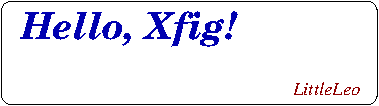
\includegraphics{hello}
  \caption*{图~1\hskip1em 这是手动编号但不出现索引中的图片的例子}
  \label{tab:badfigure3}    
\end{figure}

柳下季曰:“先生言为人父者必能诏其子,为人兄者必能教其弟,若子不听父之诏,弟不受
兄之教,虽今先生之辩,将奈之何哉?且跖之为人也,心如涌泉,意如飘风,强足以距敌,
辩足以饰非。顺其心则喜,逆其心则怒,易辱人以言。先生必无往。”

孔子不听,颜回为驭,子贡为右,往见盗跖。

\subsection{整数规划}
盗跖乃方休卒徒大山之阳,脍人肝而餔之。孔子下车而前,见谒者曰:“鲁人孔丘,闻将军
高义,敬再拜谒者。”谒者入通。盗跖闻之大怒,目如明星,发上指冠,曰:“此夫鲁国之
巧伪人孔丘非邪?为我告之:尔作言造语,妄称文、武,冠枝木之冠,带死牛之胁,多辞缪
说,不耕而食,不织而衣,摇唇鼓舌,擅生是非,以迷天下之主,使天下学士不反其本,妄
作孝弟,而侥幸于封侯富贵者也。子之罪大极重,疾走归!不然,我将以子肝益昼餔之膳。”


\chapter{其它附录}
前面两个附录主要是给本科生做例子。其它附录的内容可以放到这里,当然如果你愿意,可
以把这部分也放到独立的文件中,然后将其 \verb|\input| 到主文件中。
%\end{appendix}

% 个人简历
%\begin{resume}

  \resumeitem{个人简历}

  xxxx 年 xx 月 xx 日出生于 xx 省 xx 县。
  
  xxxx 年 9 月考入 xx 大学 xx 系 xx 专业,xxxx 年 7 月本科毕业并获得 xx 学士学位。
  
  xxxx 年 9 月免试进入 xx 大学 xx 系攻读 xx 学位至今。

  \resumeitem{发表的学术论文} % 发表的和录用的合在一起

  \begin{enumerate}[{[}1{]}]
  \item Yang Y, Ren T L, Zhang L T, et al. Miniature microphone with silicon-
    based ferroelectric thin films. Integrated Ferroelectrics, 2003,
    52:229-235. (SCI 收录, 检索号:758FZ.)
  \item 杨轶, 张宁欣, 任天令, 等. 硅基铁电微声学器件中薄膜残余应力的研究. 中国机
    械工程, 2005, 16(14):1289-1291. (EI 收录, 检索号:0534931 2907.)
  \item 杨轶, 张宁欣, 任天令, 等. 集成铁电器件中的关键工艺研究. 仪器仪表学报,
    2003, 24(S4):192-193. (EI 源刊.)
  \item Yang Y, Ren T L, Zhu Y P, et al. PMUTs for handwriting recognition. In
    press. (已被 Integrated Ferroelectrics 录用. SCI 源刊.)
  \item Wu X M, Yang Y, Cai J, et al. Measurements of ferroelectric MEMS
    microphones. Integrated Ferroelectrics, 2005, 69:417-429. (SCI 收录, 检索号
    :896KM.)
  \item 贾泽, 杨轶, 陈兢, 等. 用于压电和电容微麦克风的体硅腐蚀相关研究. 压电与声
    光, 2006, 28(1):117-119. (EI 收录, 检索号:06129773469.)
  \item 伍晓明, 杨轶, 张宁欣, 等. 基于MEMS技术的集成铁电硅微麦克风. 中国集成电路, 
    2003, 53:59-61.
  \end{enumerate}

  \resumeitem{研究成果} % 有就写,没有就删除
  \begin{enumerate}[{[}1{]}]
  \item 任天令, 杨轶, 朱一平, 等. 硅基铁电微声学传感器畴极化区域控制和电极连接的
    方法: 中国, CN1602118A. (中国专利公开号.)
  \item Ren T L, Yang Y, Zhu Y P, et al. Piezoelectric micro acoustic sensor
    based on ferroelectric materials: USA, No.11/215, 102. (美国发明专利申请号.)
  \end{enumerate}
\end{resume}

\end{document}
